\documentclass{osa-article}

%% Select the journal you're submitting to
%% oe, boe, ome, osac, osajournal
\journal{osac}
% Key:
% Express journals must have the correct journal selected:
% {oe} Optics Express
% {boe} Biomedical Optics Express
% {ome} Optical Material Express
% {osac} OSAC Continuum
% Other OSA journals may use:
% {osajournal} Applied Optics, Advances in Optics and Photonics, Journal of the Optical Society of America A/B, Optics Letters, Optica, Photonics Research

% Uncomment if submitting to Photonics Research.
% ONLY APPLICABLE FOR \journal{osajournal}
% \setprjcopyright

% Set the article type
\articletype{Research Article}
% Note that article type is not required for Express journals (OE, BOE, OME and OSAC)
\usepackage{graphicx}
\usepackage{subcaption}
\usepackage{multirow}
\usepackage{array}
\usepackage{amssymb}
\usepackage{float}
%\usepackage{amsthm}
\usepackage{amsmath}
\usepackage{lineno}
\usepackage{soul}
\usepackage{color}
\begin{document}

\title{Microring flower-like structure- Part II: designing multiplexer, half adder/subtractor and comparator circuits}

\author{Mohammad Seifi Laleh,\authormark{1} and Mohammad Razaghi,\authormark{1,*}}

\address{\authormark{1}Dept. of Electrical Engineering, University of Kurdistan, Sanandaj, Iran}

\email{\authormark{*}m.razaghi@uok.ac.ir} %% email address is required

% \homepage{http:...} %% author's URL, if desired

%%%%%%%%%%%%%%%%%%% abstract %%%%%%%%%%%%%%%%
%% [use \begin{abstract*}...\end{abstract*} if exempt from copyright]

\begin{abstract}
Designing of all-optical time-division multiplexer (TDM) and all-optical half adder/subtractor and single bit comparator circuits are presented by using GaAs–AlGaAs-based flower-like structure. These MRRs are modulated through optical pump pulses (OPPs). The OPPs are green lasers with resonant wavelength of 532 nm. Signal flow graph (SFG) method is used to theoretically analyze flower-like structure. This paper investigates new TDM topology with cross-couplings between common microring resonators (MRRs). The performance of flower-like structure is investigated by calculating some figure of merits of the resulting data streams. They show appropriate distinguishing between 0 and 1 levels of the proposed scheme’s output. This reconfigurable structure is simple, extendable, and compact and can be useful for high speed optical networks. 
\end{abstract}

%%%%%%%%%%%%%%%%%%%%%%%%%%  body  %%%%%%%%%%%%%%%%%%%%%%%%%%
\section{Introduction}
\label{}
Optical communication networks need ultra-fast logic circuits to obtain what is impossible using conventional electronics circuits. However, optical circuits suffer critical limitations in terms of compactness and power requirements. Optical processing system is a promising scheme to overcome such issues. Four wave mixing \cite{hu2014all}, nonlinear loop mirror combined photonic crystal \cite{sharma2015numerical}, triangular fiber coupler \cite{menezes2012numerical}, Mach-Zehnder (MZI) with semiconductor optical amplifier (SOA) \cite{kotb2017performance}, \cite{kotb2018all} and microring resonator-based (MRR) structures \cite{lalehsimulation}, \cite{rakshit2014micro} are approaches to realize all-optical logic gates for high speed processing systems. Controlling light by light is a well-known method to achieve optical switches \cite{rakshit2013design}. Here, the optical pump pulse (OPP) is used to change the optical properties of a nonlinear medium \cite{wang2012simulative}. In MZI with SOA \cite{dimitriadou2013feasibility}, providing nonlinear media is a duty of SOA, \cite{houbavlis2003soa}, while the MRR material systems providing nonlinearity which is required to make an optical switch \cite{li2012theoretical}, \cite{heebner1999enhanced}. Thus MRR-based structures do never need any electrically contacted gain into the cavity.\\
Optical MRRs have been used in wide range research progresses of optical science, such as all-optical nonlinear switching \cite{forst2007high}, optical gates \cite{ibrahim2003all}, modulators \cite{tazawa2006ring}, biosensors \cite{de2007silicon}, optical filters \cite{tobing2008boxlike}, microlasers \cite{benson2006micro}, Raman lasing \cite{de2013design}, and  elements of all-optical signal processing \cite{van2002optical}.\\
Multiplexing \cite{schwelb2006crosstalk} is an essential feature of optical processing systems in which a great quantity of information is transmitted with no mutual disturbances. Optical multiplexers are able to combine several channels into a single channel to transmit by optical networks. There are several schemes to realize optical multiplexers \cite{wu2012proposal} such as polarization diversity \cite{shen2008reconfigurable}, twisting of the nonlinear fiber \cite{xu2011reconfigurable}, depolarization of the clock pulses \cite{ismail2011all}, cross-phase modulation (XPM) effect \cite{lin1999investigation}, multilayer interference filters \cite{roy2014design},  fiber Bragg grating filters \cite{zoiros2005complete} and MRR-based structures \cite{lalehsimulation}, \cite{rakshit2013design}.\\
 Also, all-optical adder/subtractor and comparator units build high-speed digital optical micro-operations. These circuits have many applications in optical computing and information processing. In this paper we have designed special nonlinear structures based on flower-like MRRs configuration \cite{razaghi2016design} to obtain time-division multiplexer (TDM), half adder/subtractor and single bit comparator. The proposed flower-like structure has novelties such as its all-optical nature, using only MRRs to design a high quality factor, monolithically integrated, enhanced operational bandwidth and reduced power consumption optical gates \cite{laleh2019performance}. Also, the proposed structure can easily be extended for higher order inputs by adding more petals or by serially/parallel coupling some flower-like structures to each other \cite{razaghi2016design}.\\
The paper is organized as follows: Operational principle of all-optical TDM using flower-like structure is discussed in Section 2. In Section 3, simulation results and discussion of the proposed scheme for TDM, half adder/subtractor and single bit comparator are explained and Section 4 is a conclusion of the paper.

\section{ Operational principle of all-optical TDM using flower-like structure}
\label{} 
Fig.\ref{fig1_flower} shows a four-petal flower-like structure in GaAs-AlGaAs material system. The central MRR (3$^{\text{rd}}$ MRR) has never been pumped by any OPP. The MRR$_1$, MRR$_2$, MRR$_4$ and MRR$_5$ are pumps by \textit{OPP A}, \textit{OPP B}, \textit{OPP $B'$} and \textit{OPP $A'$}.
\begin{figure}[tb]
\centering
	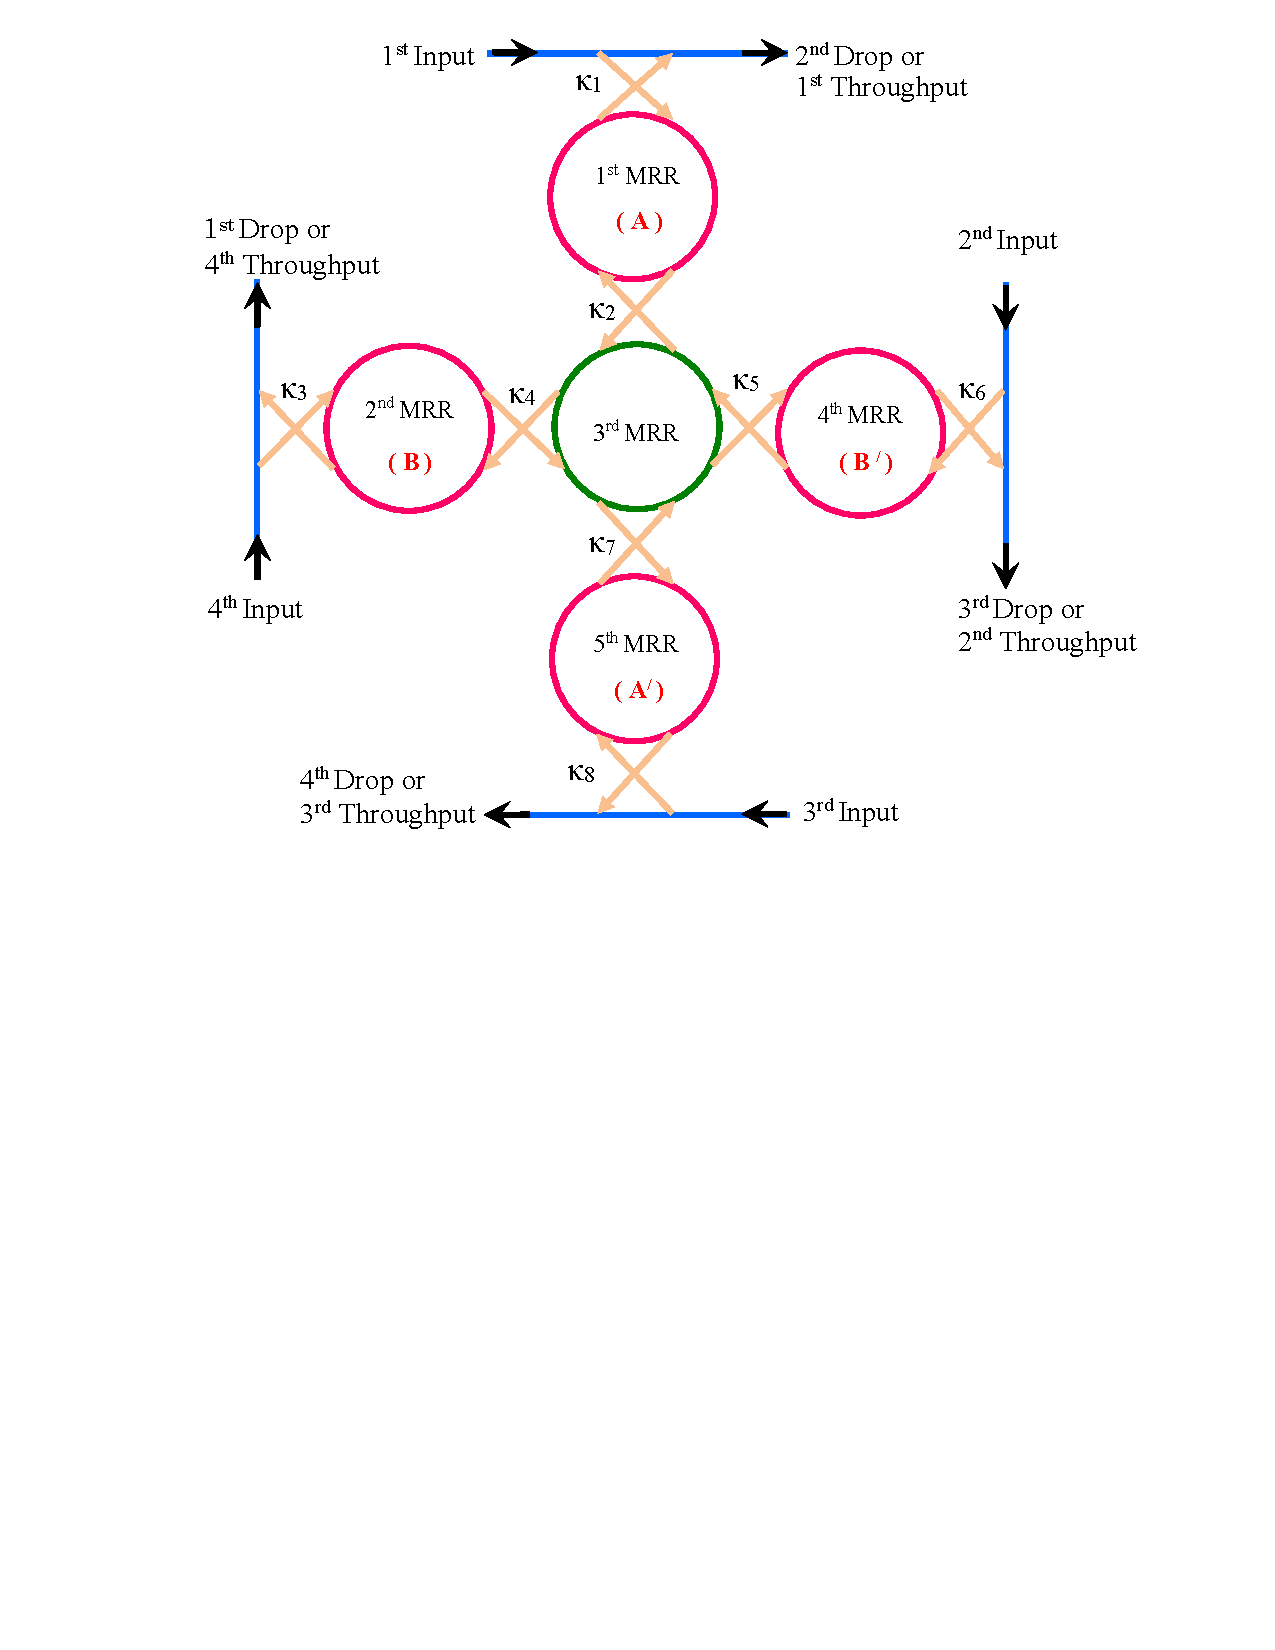
\includegraphics[width=4 in]{figs/fig1_flower.pdf}
	\caption{Schematic of an flower-like structure.}
	\label{fig1_flower}
\end{figure}
 The effect of cross-coupling and average peak power have been considered to calculate transfer functions and to obtain required average peak power to make refractive index of MRRs changed. In the proposed structure when light is applied to an input port, it might be extracted at each drop port of the other waveguides or removed from its throughput port. Defining all parameters and calculating transfer function from the specified input port (1$^{\text{st}}$ input port) to the 1$^{\text{st}}$, the 3$^{\text{rd}}$ and the 4$^{\text{th}}$ drop port are explained in Appendix. Calculation the other transfer functions are same as what has been presented in Appendix. Also, Flower-like structure is extendable. It could be extended by adding more petals or by serially/parallel coupled some flower-like structures \cite{razaghi2016design}. Now, we represent cases in which optical signal has been injected in the only one input port and it would be extracted from optimum drop port. In fact, there are some optical paths that experience less optical losses \cite{razaghi2016design}. They have less effective optical path from an input port to the desired drop port. The optimum routs in flower-like structure have been explained in ref \cite{razaghi2016design}. These cases are introduced based on states of \textit{OPP (A)} and \textit{OPP (B)} in Tab. \ref{tab1}.
  \begin{table}[H]
\caption{All optimum input - drop ports of flower-like structure based on the OPP (\textit {A}), OPP (\textit {B}) values.}
\centering 
\resizebox{\textwidth}{!}{%
\begin{tabular}{c|c|c|c|c|c|c|c|c|c|c}
\hline\hline
\multirow{2}{*}{A}& \multirow{2}{*}{B}& \multirow{2}{*}{Input port}& \multicolumn{5}{c|}{Resonance status of MRRs}& \multirow{2}{*}{Forward path}& \multirow{2}{*}{Drop port}& \multirow{2}{*}{Optical gate}\\
\cline{4-8}
& & & 1$^{\text{st}}$& 2$^{\text{nd}}$& 3$^{\text{rd}}$& 4$^{\text{th}}$& 5$^{\text{th}}$& & &\\
\hline
0&0& 1$^{\text{st}}$& on& on& on& off& off& 1-3-2& 1$^{\text{st}}$& $A'$.$B'$\\ 
%\cline{3-11}
%& & 2$^{\text{nd}}$& N.A& N.A& on& off& N.A& -& 3$^{\text{rd}}$& $B'$\\
%\cline{3-11}
%& & 3$^{\text{rd}}$& N.A& N.A& on& N.A& off& -& 4$^{\text{th}}$& $A'$\\
%\cline{3-11}
%& & 4$^{\text{th}}$& on& on& on& off& off& 2-3-1& 2$^{\text{nd}}$& $A'$.$B'$\\
\hline 
0&1&  2$^{\text{nd}}$& on& off& on& on& off& 4-3-1& 2$^{\text{nd}}$& $A'$.\textit B\\
%\cline{3-11}
%& & 2$^{\text{nd}}$& on& off& on& on& off& 4-3-1& 2$^{\text{nd}}$& $A'$.\textit B\\
%\cline{3-11}
%& & 3$^{\text{rd}}$& N.A& N.A& on& N.A& off& -& 4$^{\text{th}}$& $A'$\\
%\cline{3-11}
%& & 4$^{\text{th}}$& N.A& off& on& N.A& N.A& -& 1$^{\text{st}}$& \textit B\\
\hline
1&0& 4$^{\text{th}}$& off& on& on& off& on& 2-3-5& 4$^{\text{th}}$& \textit A.$B'$\\
%\cline{3-11}
%& & 2$^{\text{nd}}$& N.A& N.A& on& off& N.A& -& 3$^{\text{rd}}$& $B'$\\
%\cline{3-11}
%& & 3$^{\text{rd}}$& off& on& on& off& on& 5-3-2& 1$^{\text{st}}$& \textit A.$B'$\\
%\cline{3-11}
%& & 4$^{\text{th}}$& off& on& on& off& on& 2-3-5& 4$^{\text{th}}$& \textit A.$B'$\\
\hline 
1&1& 3$^{\text{rd}}$& off& off& on& on& on& 5-3-4& 3$^{\text{rd}}$& \textit A.\textit B\\
%\cline{3-11}
%& & 2$^{\text{nd}}$& off& off& on& on& on& 4-3-5& 4$^{\text{th}}$& \textit A.\textit B\\
%\cline{3-11}
%& & 3$^{\text{rd}}$& off& off& on& on& on& 5-3-4& 3$^{\text{rd}}$& \textit A.\textit B\\
%\cline{3-11}
%& & 4$^{\text{th}}$& N.A& off& on& N.A& N.A& -& 1$^{\text{st}}$& \textit B\\
\hline 
\end{tabular}
}
\label{tab1} % is used to refer this table in the text
\end{table}
A flower-like based 4:1 TDM is depicted in Fig.\ref{fig2_combiner}. Here, four different input signals have been applied to the input ports of flower-like structure. All drop ports of flower-like structure are combined to make TDM output signal. The beam combiner gets four drop port signals of flower-like MRRs to achieve reconfigurable logic gates \cite{bloembergen1996nonlinear}, \cite{shen1984principles}. The \textit{OPP A} and \textit{OPP B} are selection legs by which optical signal of an input port is chosen to transmit on the TDM output port. 
\begin{figure}
\centering
	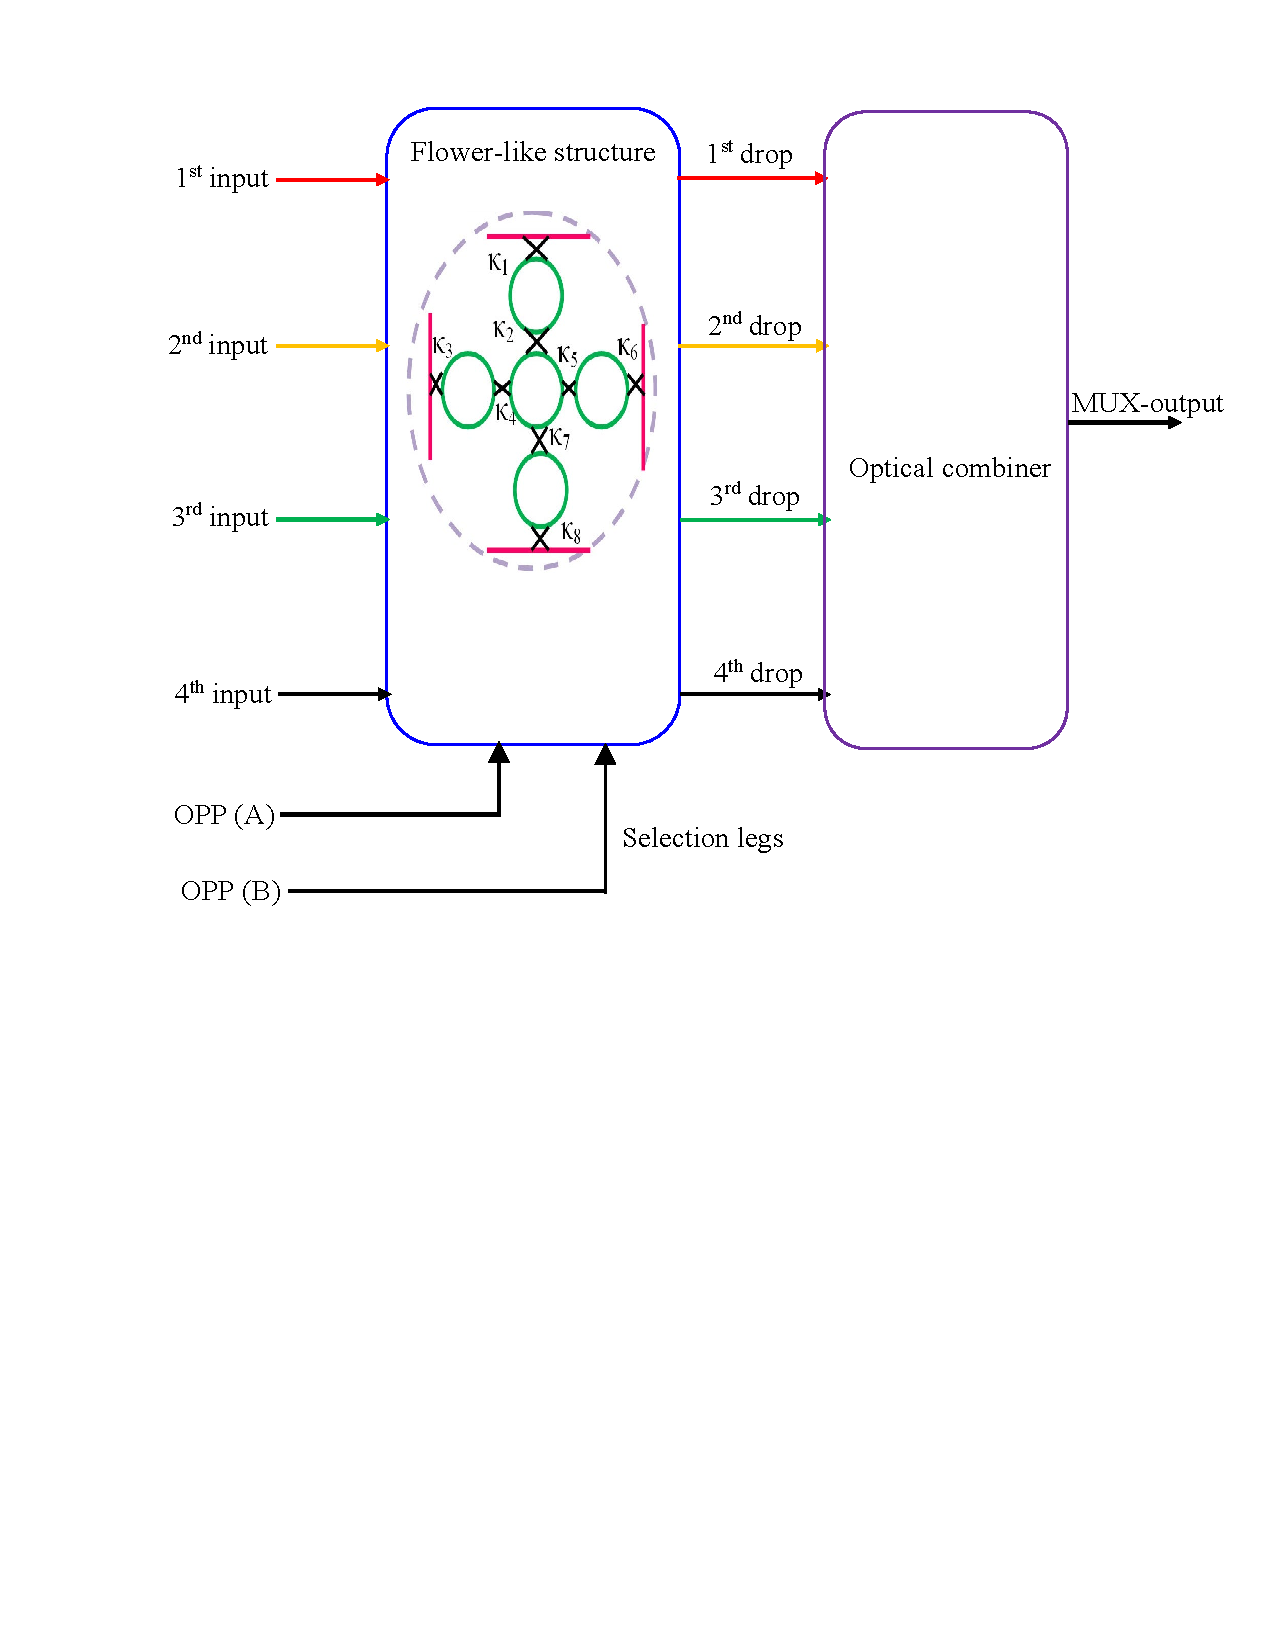
\includegraphics[width=3.5 in]{figs/fig2_combiner.pdf}
	\caption{A 4:1 TDM based on flower-like structure}
	\label{fig2_combiner}
\end{figure}
Table \ref{tab2} shows input/drop port signals of flower-like structure when selection legs \textit{OPP A}=0 and \textit{OPP B}=0.

  \begin{table}[H]
\caption{Possible optical signals at drop ports of flower-like structure in the case that  OPP (\textit {A})=0 and OPP (\textit {B})=0.}
\centering 
\resizebox{\textwidth}{!}{%
\begin{tabular}{c|c|c|c|c|c|c|c|c|c|c}
\hline\hline
\multirow{2}{*}{A}& \multirow{2}{*}{B}& \multirow{2}{*}{Input port}& \multicolumn{5}{c|}{Resonance status of MRRs}& \multirow{2}{*}{Forward path}& \multirow{2}{*}{Drop port}& \multirow{2}{*}{Optical gate}\\
\cline{4-8}
& & & 1$^{\text{st}}$& 2$^{\text{nd}}$& 3$^{\text{rd}}$& 4$^{\text{th}}$& 5$^{\text{th}}$& & &\\
\hline
\multirow{4}{*}{0}& \multirow{4}{*}{0}& 1$^{\text{st}}$& on& on& on& off& off& 1-3-2& 1$^{\text{st}}$& 1$^{\text{st}}$input.$A'$.$B'$\\ 
\cline{3-11}
& &1$^{\text{st}}$& on& N.A& on& N.A& N.A& -& 2$^{\text{nd}}$& No signal\\ 
%& & 2$^{\text{nd}}$& N.A& N.A& on& off& N.A& -& 3$^{\text{rd}}$& $B'$\\
\cline{3-11}
& & 1$^{\text{st}}$& on& N.A& on& off& N.A& -& 3$^{\text{rd}}$& No signal\\ 
%& & 3$^{\text{rd}}$& N.A& N.A& on& N.A& off& -& 4$^{\text{th}}$& $A'$\\
\cline{3-11}
& & 1$^{\text{st}}$& on& N.A& on& N.A& off& -& 4$^{\text{th}}$& No signal\\
%& & 4$^{\text{th}}$& on& on& on& off& off& 2-3-1& 2$^{\text{nd}}$& $A'$.$B'$\\
\hline 
\multirow{4}{*}{0}& \multirow{4}{*}{0}& 2$^{\text{nd}}$&N.A& on& on& off& N.A& -& 1$^{\text{st}}$& No signal\\ 
\cline{3-11}
& & 2$^{\text{nd}}$& on& N.A& on& off& N.A& -& 2$^{\text{nd}}$& No signal\\
\cline{3-11}
& & 2$^{\text{nd}}$& N.A& N.A& on& off& N.A& -& 3$^{\text{rd}}$& $B'$\\
%& & 3$^{\text{rd}}$& N.A& N.A& on& N.A& off& -& 4$^{\text{th}}$& $A'$\\
\cline{3-11}
& & 2$^{\text{nd}}$& N.A& N.A& on& off& off& -& 4$^{\text{th}}$& No signal\\
%& & 4$^{\text{th}}$& N.A& off& on& N.A& N.A& -& 1$^{\text{st}}$& \textit B\\
\hline
\multirow{4}{*}{0}& \multirow{4}{*}{0}& 3$^{\text{rd}}$& N.A& on& on& N.A& off& -& 1$^{\text{st}}$& No signal\\
\cline{3-11}
& & 3$^{\text{rd}}$& on& N.A& on&N.A& off& -& 2$^{\text{nd}}$& No signal\\
%& & 2$^{\text{nd}}$& N.A& N.A& on& off& N.A& -& 3$^{\text{rd}}$& $B'$\\
\cline{3-11}
& & 3$^{\text{rd}}$& N.A& N.A& on&off& off& -& 3$^{\text{rd}}$& No signal\\
%& & 3$^{\text{rd}}$& off& on& on& off& on& 5-3-2& 1$^{\text{st}}$& \textit A.$B'$\\
\cline{3-11}
& & 3$^{\text{rd}}$& N.A& N.A& on& N.A& off& -& 4$^{\text{th}}$& $A'$\\
%& & 4$^{\text{th}}$& off& on& on& off& on& 2-3-5& 4$^{\text{th}}$& \textit A.$B'$\\
\hline 
\multirow{4}{*}{0}& \multirow{4}{*}{0}& 4$^{\text{th}}$& N.A& on& on& N.A& N.A&-& 1$^{\text{st}}$& No signal\\
\cline{3-11}
& & 4$^{\text{th}}$& on& on& on& off& off& 2-3-1& 2$^{\text{nd}}$&4$^{\text{th}}$ input. $A'$.$B'$\\
%& & 2$^{\text{nd}}$& off& off& on& on& on& 4-3-5& 4$^{\text{th}}$& \textit A.\textit B\\
\cline{3-11}
& & 4$^{\text{th}}$& N.A& on& on& off& N.A& -& 3$^{\text{rd}}$& No signal\\ 
%& & 3$^{\text{rd}}$& off& off& on& on& on& 5-3-4& 3$^{\text{rd}}$& \textit A.\textit B\\
\cline{3-11}
& & 4$^{\text{th}}$& N.A& on& on& N.A& off& -& 4$^{\text{th}}$& No signal\\
\cline{3-11}
& & 4$^{\text{th}}$& N.A& off& on& N.A& N.A& -& 1$^{\text{st}}$& \textit B\\
\hline 
\end{tabular}
}
\label{tab2} % is used to refer this table in the text
\end{table}

It could be seen for selection legs \textit{A}\textit{B}=00 optical signal of the input/drop ports (1-1)+(4-2) are extracted at the output of TDM. Same as Table \ref{tab2} in cases where selection legs are  \textit{A}\textit{B}=01,  \textit{A}\textit{B}=10 and  \textit{A}\textit{B}=11 optical signal of the input/drop ports (2-2)+(1-3), (4-4)+(3-1) and (3-3)+(2-4) have been extracted at output of TDM respectively. All these cases have been investigated in subsequent section.\\
In this paper extinction ratio (\textit {ER}), contrast ratio (\textit {CR}) , amplitude modulation factor (\textit {AM}) and eye opening factor (\textit {EO}) are calculated for operational logic gates \cite{houbavlis2004performance}. These figure of merits have been defined as follow :
\begin{equation}
ER(dB)=10log\frac{P^1_{min}} {P^0_{max}}
\label{eq:1}
\end{equation}

 \begin{equation}
CR(dB)=10log\frac{P^1_{mean}} {P^0_{mean}}
\label{eq:2}
\end{equation}

\begin{equation}
AM(dB)=10log\frac{P^1_{max}} {P^1_{min}}
\label{eq:3}
\end{equation}
 
\begin{equation}
EO=\frac{P^1_{min}-P^0_{max}} {P^1_{min}}
\label{eq:4}
\end{equation}

where, \textit {P$^1_{min}$} and \textit {P$^1_{max}$} are the minimum and maximum values of the peak intensity of high (`1') level. $P^1_{mean}$ and $P^0_{mean}$ are mean value of output intensity for high (`1') and low (`0') levels. Also, \textit {P$^0_{max}$} is the maximum value of intensity at low level (`0'). The $CR$ and $ER$ should be greater than 10 dB and \textit{AM} need to be lower than 1 dB. Also, high value of \textit{EO} determines quality of clear transmission.

\section{RESULTS AND DISCUSSIONS}
\label{}

To simulate flower-like structure all parameters such as effective waveguide cross section, MRR’s radii, resonance wavelength of MRRs, internal and external coupling coefficients, and gap between all elements in structure (waveguide and MRRs)  are same as what have been defined in \cite{lalehsimulation}. Also, OPPs are green lasers of wavelength 532 nm with average power of 2.29 mW and optical pulse bit rate is 10 Gbit/s. Here, Simulation is done based on the string of bits for \textit{OPP A} and \textit{OPP B} as 00001111 and 00110011. All results have been achieved using Gaussian shape input pulses with peak power of 0.2 mW and pulse width of 2 ps. These values have been chosen to overcome undesired pumping procedure during injection optical signals through input ports \cite{lalehsimulation}. Additionally, programming environment of MATLAB software is used to calculate all transfer functions.
First of all, we simulate a TDM, being shown in Fig.\ref{fig2_combiner}. There are four different optical signals at input ports of flower-like structure. The 1$^{\text{st}}$ input is binary string 11000000, the 2$^{\text{nd}}$ input is 00100000, the 3$^{\text{rd}}$ and the 4$^{\text{th}}$ inputs are 00001100 and 00000001. Simulation results are presented in Fig.\ref{fig3_muxfi}. It can be seen that output of TDM is the string consists all input signals. Important parameters of TDM have been represented in Table \ref{tab3}.
\begin{figure}[tb]
\centering
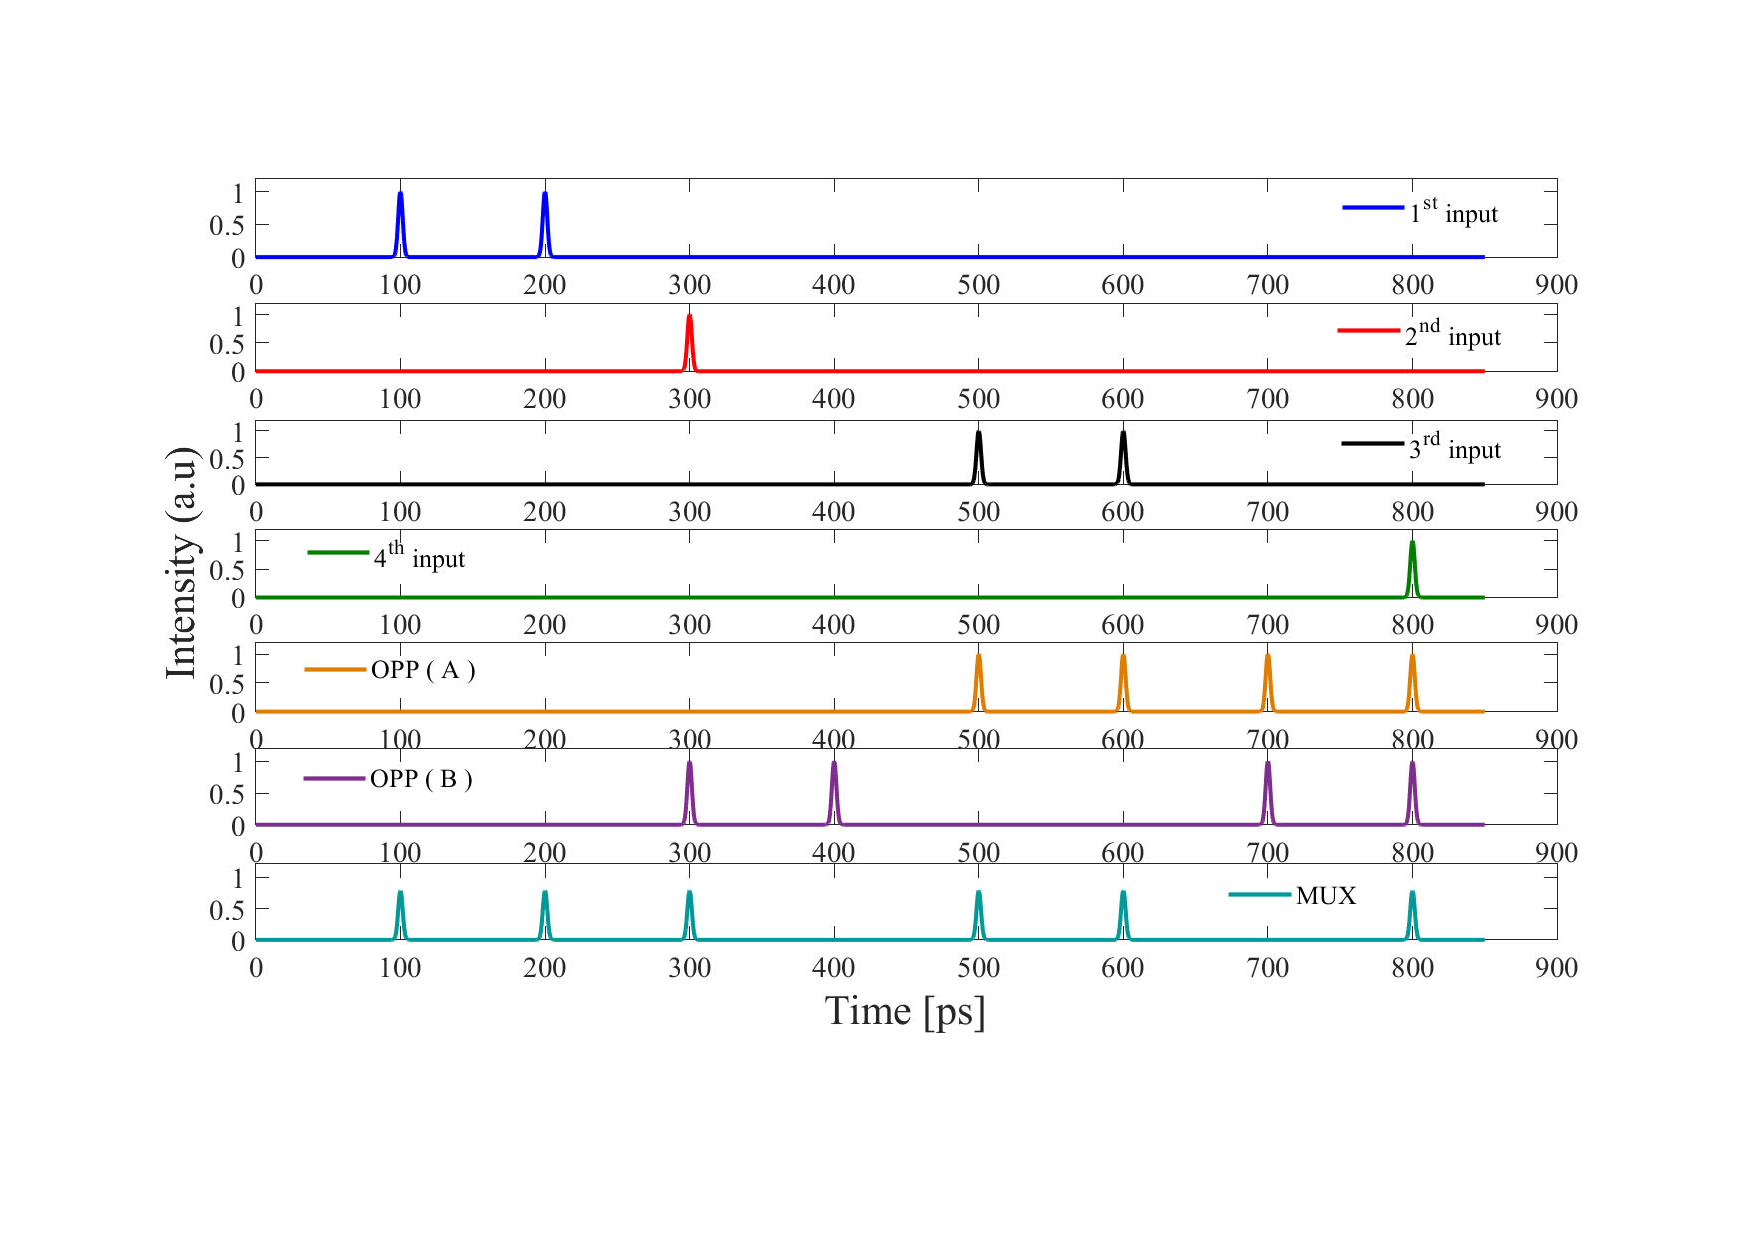
\includegraphics[width=5 in]{figs/fig3_muxfi.pdf}
	\caption{Simulation result of optical comparator.}
	\label{fig3_muxfi}
\end{figure}

\begin{table}[H]
\caption{Logical truth table of the proposed TDM and OPP levels at the input and output (N.A = do not care).}
\centering 
\resizebox{\textwidth}{!}{%
\begin{tabular}{c|c|c|c|c|c|c|c|c|c}
\hline\hline
\multirow{2}{*}{A}& \multirow{2}{*}{B}& \multirow{2}{*}{Input port}& \multicolumn{4}{c|}{Status of input signals [mW]}& \multirow{2}{*}{Forward path}& \multirow{2}{*}{Drop port}& \multirow{2}{*}{TDM's output [mW]}\\
\cline{4-7}
& & & 1$^{\text{st}}$& 2$^{\text{nd}}$& 3$^{\text{rd}}$& 4$^{\text{th}}$& & &\\
\hline
\multirow{2}{*}{0}& \multirow{2}{*}{0}& 1$^{\text{st}}$& 2.29&N.A& N.A& N.A& 1-3-2& 1$^{\text{st}}$& 0.15748\\ 
\cline{3-10}
& & 4$^{\text{th}}$& N.A& N.A& N.A& 2.29&2-3-1& 2$^{\text{nd}}$& 0\\
\hline 
\multirow{2}{*}{0}& \multirow{2}{*}{1}& 2$^{\text{nd}}$& N.A& 2.29& N.A& N.A&4-3-1& 2$^{\text{nd}}$& 0.15622\\ 
\cline{3-10}
& & 1$^{\text{st}}$& 2.29& N.A& N.A& N.A& 1-3-4& 3$^{\text{rd}}$& 0\\
\hline
\multirow{2}{*}{1}& \multirow{2}{*}{0}& 3$^{\text{rd}}$& N.A& N.A& 2.29& N.A&5-3-4& 3$^{\text{rd}}$& 0.15681\\ 
\cline{3-10}
& & 2$^{\text{nd}}$& N.A& 2.29& N.A& N.A&4-3-5& 4$^{\text{th}}$&0\\
\hline 
\multirow{2}{*}{1}& \multirow{2}{*}{1}& 4$^{\text{th}}$& N.A& N.A & N.A& 2.29&2-3-5& 4$^{\text{th}}$& 0.15714\\ 
\cline{3-10}
& & 3$^{\text{rd}}$& N.A& N.A& 2.29& N.A& 5-3-2& 1$^{\text{st}}$& 0\\
\hline 
\end{tabular}
}
\label{tab3} % is used to refer this table in the text
\end{table}

Comparison between two binary data is required to control or drive the physical variable on the basis of a reference value. The flower-like structure can compare two binary bites and generates one of the outputs \textit {A} =\textit {B}, \textit {A}$>$\textit {B} and \textit {A}$<$\textit {B}. To obtain a comparator circuit, the \textit{XNOR} and \textit{AND} gates would be used. The \textit{XNOR} gate is used in the cases in which the binary digits are equal and the \textit{AND} gate is used through the cases that a binary digitis is greater than or less than the other one. Just based on Tab. \ref{tab4}, the binary combinator can be achieved. The simulation results have been illustrated in Fig.\ref{fig4_comparator}.\\
\begin{figure}[tb]
\centering
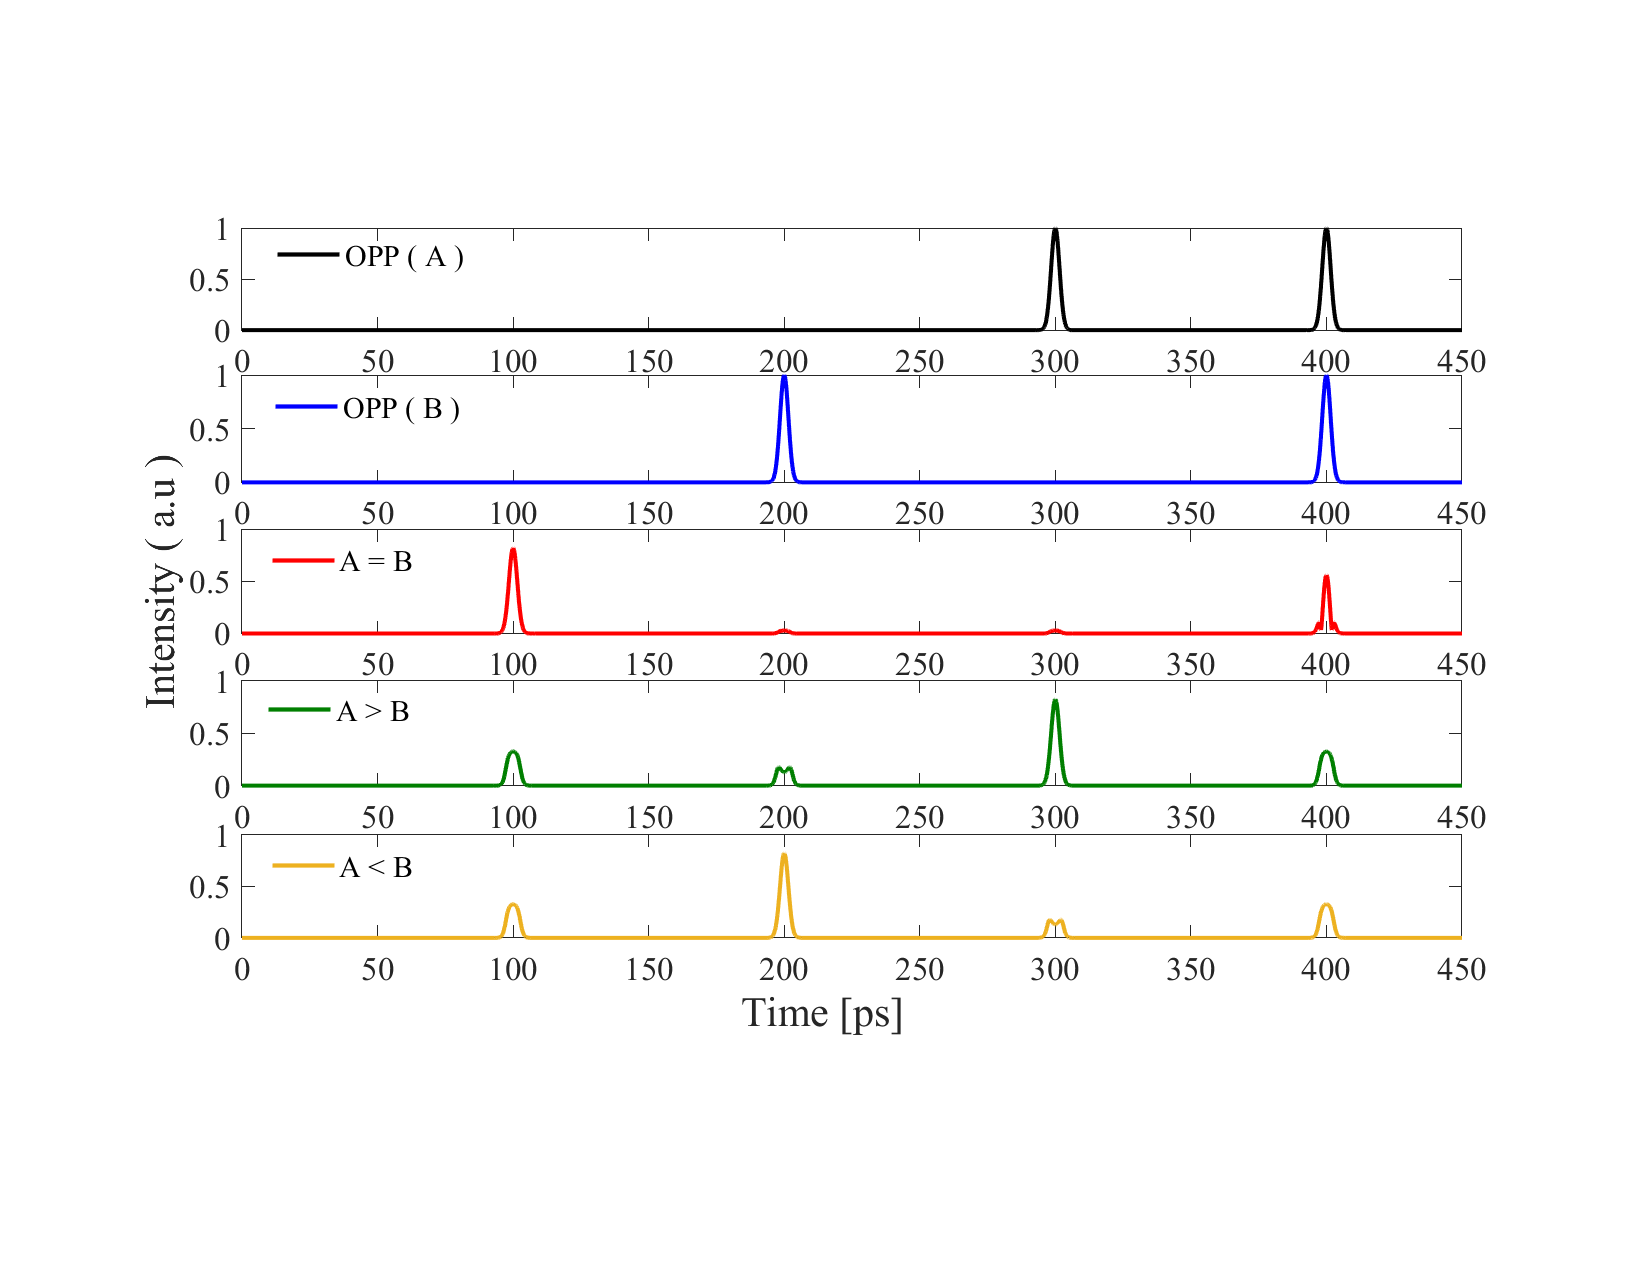
\includegraphics[width=3 in]{figs/fig4_comparator.pdf}
	\caption{Simulation result of optical comparator.}
	\label{fig4_comparator}
\end{figure}
 
\begin{table}[H]
\caption{the parameters of flower-like structure  as optical comparator.}
\centering 
\resizebox{\textwidth}{!}\\
\cline{4-5}
& & &Max&Min& & & & &\\
\hline
\multirow{2}{*}{\textit A=\textit B}&\multirow{2}{*}{$A\oplus  B$}& \multirow{2}{*}{(4-4)+(2-2)}&0.0284&0.0281&0&\multirow{2}{*}{13.291}&\multirow{2}{*}{14.024}&\multirow{2}{*}{1.319}&\multirow{2}{*}{95.31}\\
\cline{4-6}
& & &0.821&0.606&1 & & & &\\
\hline
\multirow{2}{*}{\textit A$>$\textit B}&\multirow{2}{*}{\textit A. $B'$}& \multirow{2}{*}{4-4}&0.324&0.141&0&\multirow{2}{*}{13.96}&\multirow{2}{*}{15.45}&\multirow{2}{*}{0.0853}&\multirow{2}{*}{95.98}\\
\cline{4-6}
& & &0.823&0.807&1 & & & &\\
\hline
\multirow{2}{*}{\textit A$<$\textit B}&\multirow{2}{*}{$A'$.\textit B}& \multirow{2}{*}{2-2}&0.301&0.139&0&\multirow{2}{*}{14.26}&\multirow{2}{*}{15.64}&\multirow{2}{*}{0.048}&\multirow{2}{*}{96.25}\\
\cline{4-6}
& & &0.811&0.802&1 & & & &\\
\hline
\end{tabular}
}
\label{tab4} % is used to refer this table in the text
\end{table}

The flower-like structure can be also used to design optical half adder and half subtractor. The possible combination of input/drop ports to obtain the two-inputs half adder are given in Tab. \ref{tab5}\\

\begin{table}[H]
\caption{The parameters of flower-like structure  as optical half adder.}
\centering 
\resizebox{\textwidth}{!}\\
\cline{4-5}
& & &Max&Min& & & & &\\
\hline
\multirow{2}{*}{Sum}&\multirow{2}{*}{$A\oplus B$}& \multirow{2}{*}{(4-4)+(2-2)}&0.312&0.306&0&\multirow{2}{*}{12.95}&\multirow{2}{*}{13.798}&\multirow{2}{*}{1.47}&\multirow{2}{*}{94.93}\\
\cline{4-6}
& & &0.866&0.616&1 & & & &\\
\hline
\multirow{2}{*}{Carry}&\multirow{2}{*}{\textit A.\textit B}& \multirow{2}{*}{3-3}&0.302&0.163&0&\multirow{2}{*}{14.58}&\multirow{2}{*}{15.72}&\multirow{2}{*}{0.045}&\multirow{2}{*}{96.52}\\
\cline{4-6}
& & &0.868&0.8671&1 & & & &\\
\hline
\end{tabular}
}
\label{tab5} % is used to refer this table in the text
\end{table}

Fig.\ref{fig5_adder} presents the half adder simulation results. In this case, Sum=$A'B+AB'$($A\oplus B$) and Carry=\textit {A}.\textit {B}.
   \begin{figure}[tb]
\centering
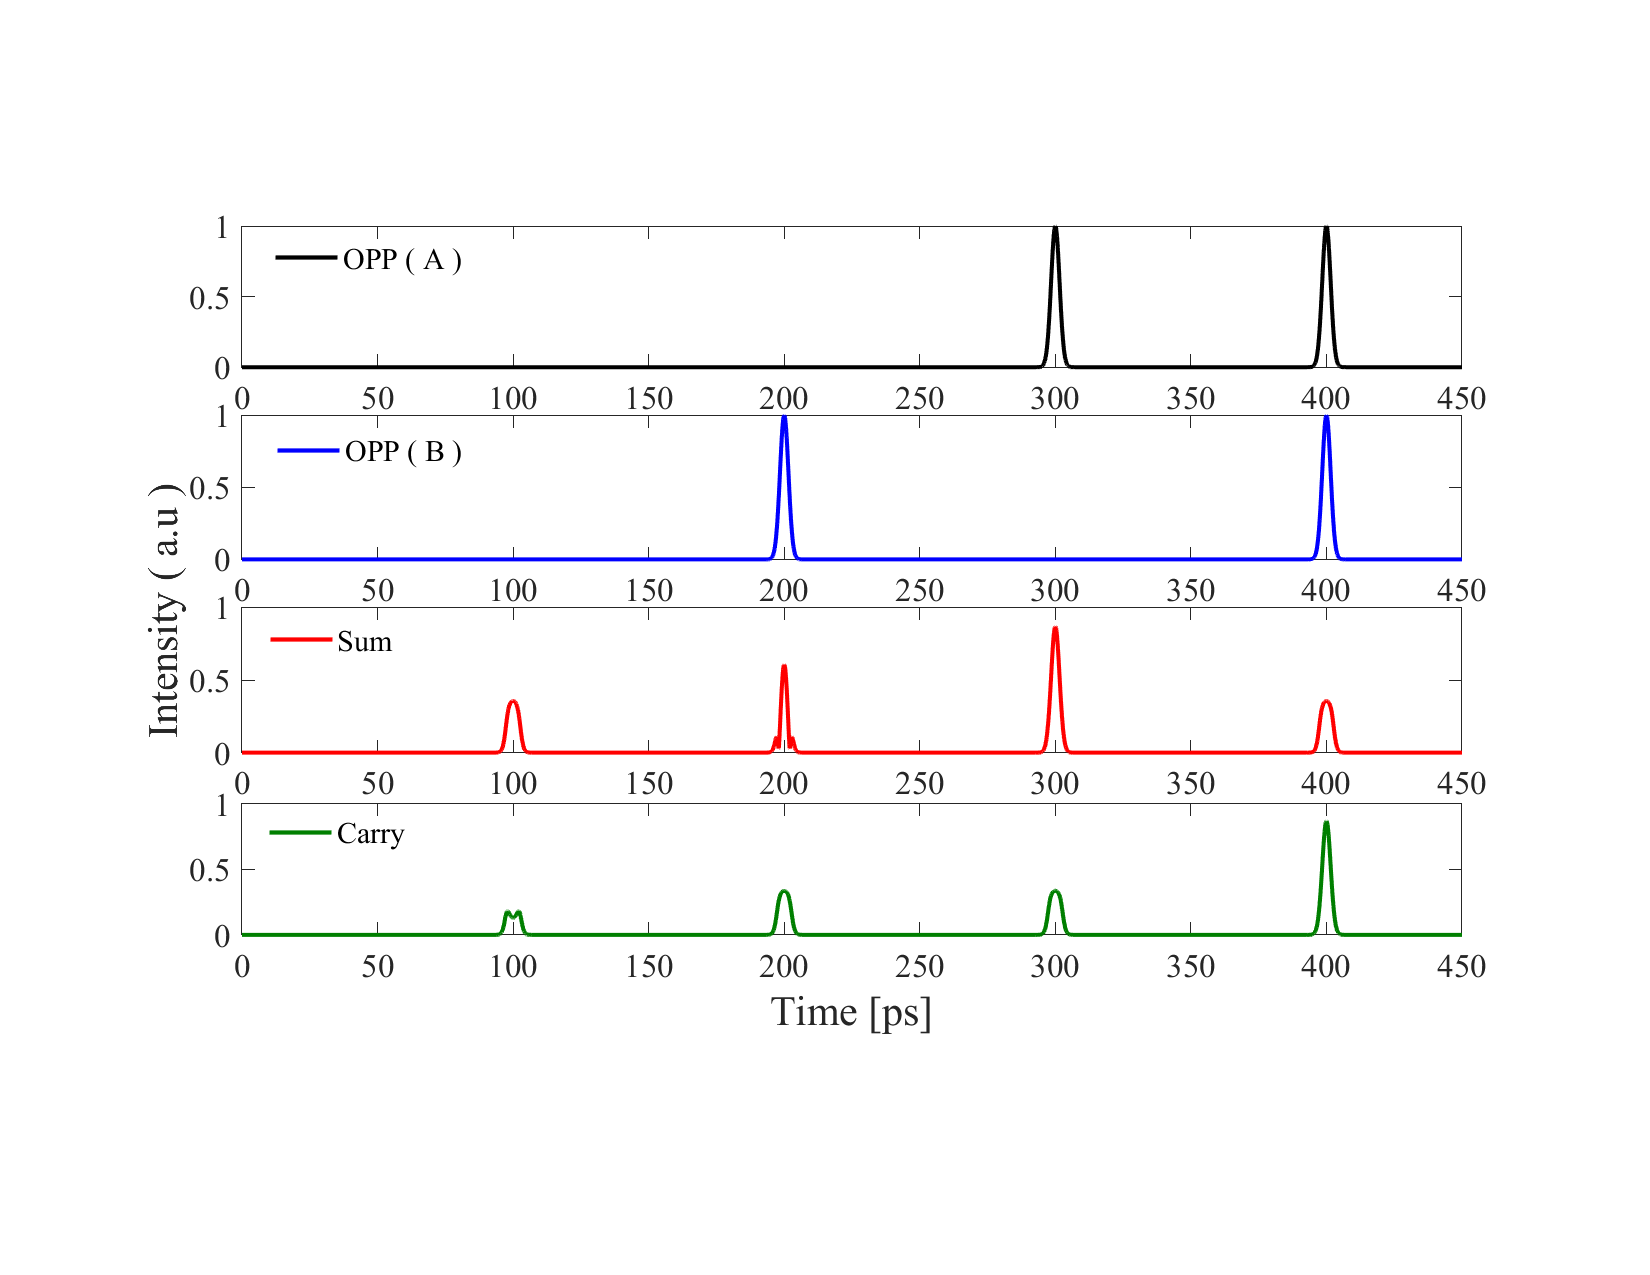
\includegraphics[width=3 in]{figs/fig5_adder.pdf}
	\caption{Simulation result of optical half adder.}
	\label{fig5_adder}
\end{figure}

The half subtractor has two outputs which can be achieved as follow. Difference=$A'$.\textit {B}+\textit {A}.$B'$ (\textit {A}$\oplus$\textit {B}) and Borrow=\textit {A}.$B'$. So, the \textit{XOR} output simultaneously gives the result of sum and difference. Simulation results of half subtractor have been shown in Fig. \ref{fig6_subtractor}. Also important output parameters are reported at Tab. \ref{tab6}.
   \begin{figure}[tb]
\centering
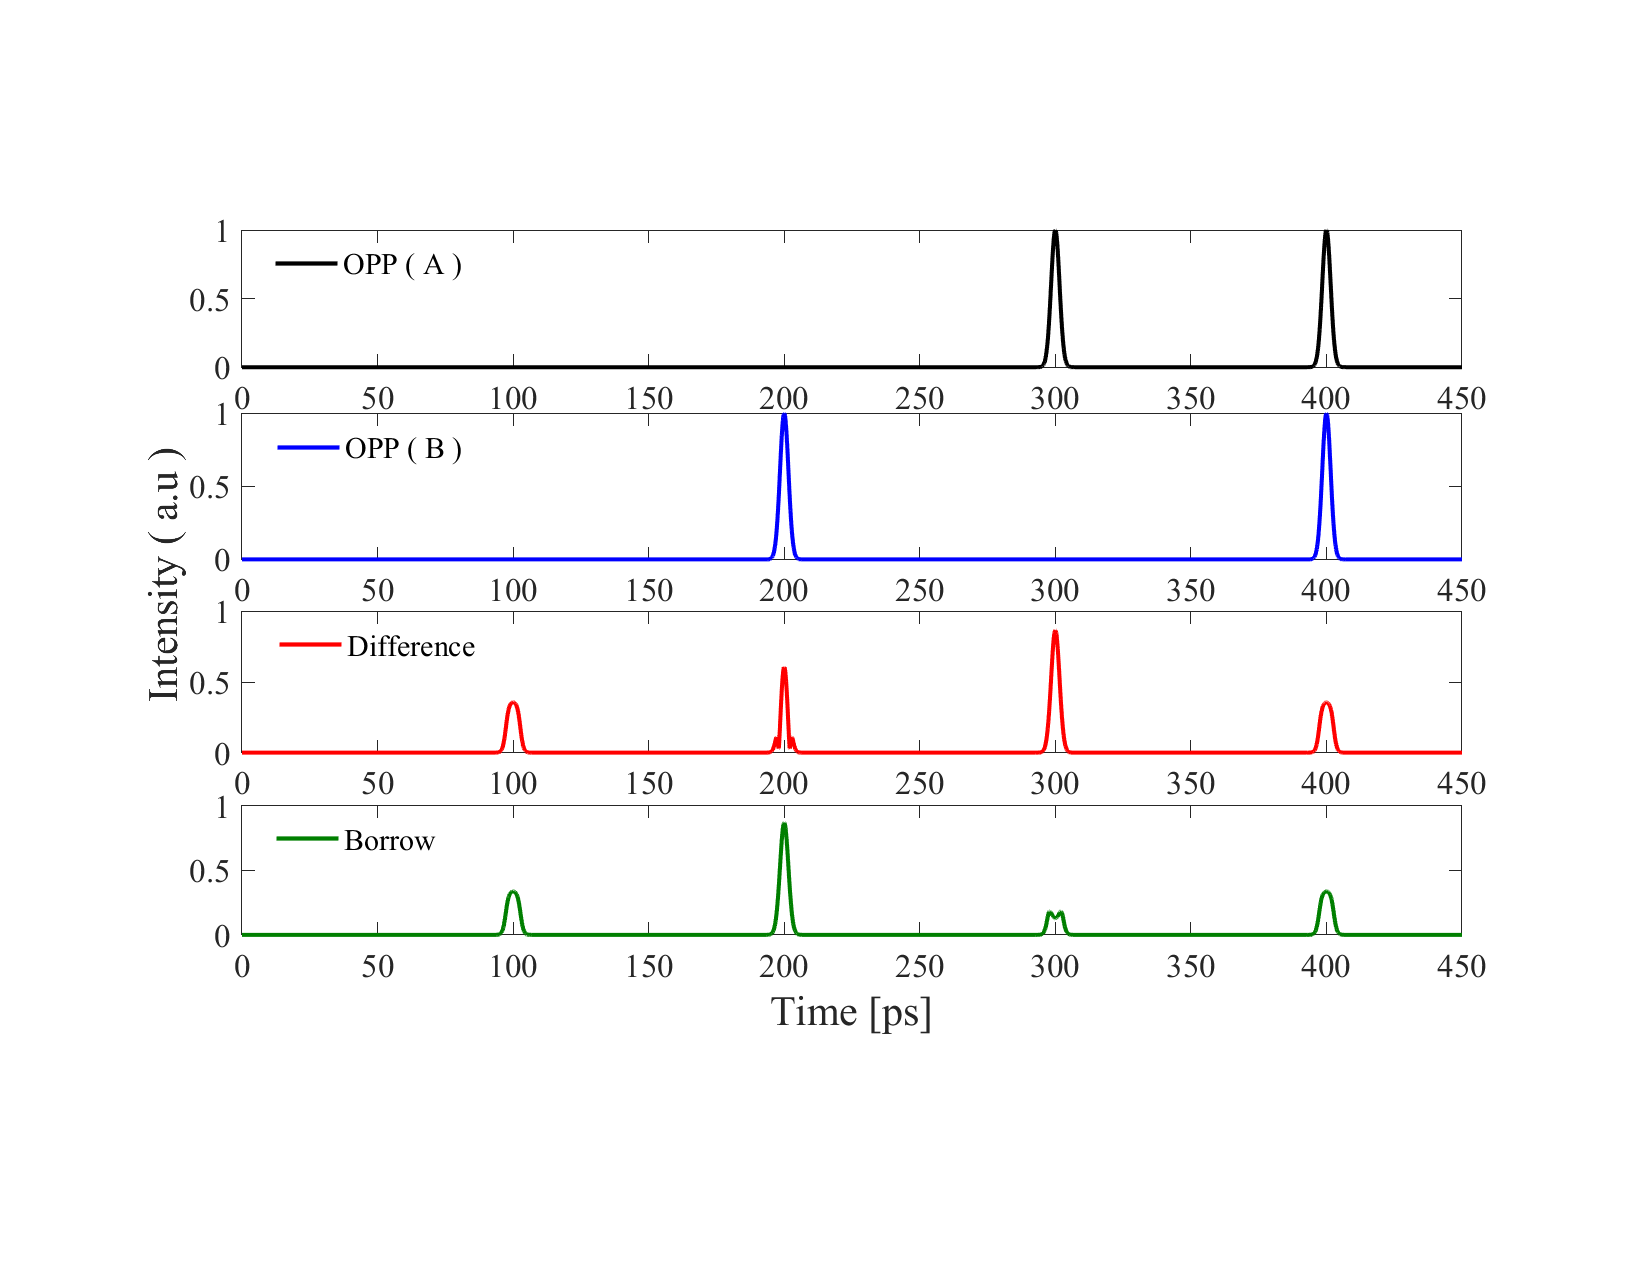
\includegraphics[width=3 in]{figs/fig6_subtractor.pdf}
	\caption{Simulation result of optical half subtractor.}
	\label{fig6_subtractor}
\end{figure}

\begin{table}[H]
\caption{The parameters of flower-like structure  as half subtractor.}
\centering 
\resizebox{\textwidth}{!}\\
\cline{4-5}
& & &Max&Min& & & & &\\
\hline
\multirow{2}{*}{Difference}&\multirow{2}{*}{$A\oplus B$}& \multirow{2}{*}{(4-4)+(2-2)}&0.336&0.335&0&\multirow{2}{*}{12.56}&\multirow{2}{*}{13.42}&\multirow{2}{*}{1.55}&\multirow{2}{*}{94.45}\\
\cline{4-6}
& & &0.867&0.606&1 & & & &\\
\hline
\multirow{2}{*}{Borrow}&\multirow{2}{*}{\textit A.$B'$}& \multirow{2}{*}{4-4}&0.318&0.171&0&\multirow{2}{*}{14.33}&\multirow{2}{*}{15.49}&\multirow{2}{*}{0.0451}&\multirow{2}{*}{96.31}\\
\cline{4-6}
& & &0.871&0.862&1 & & & &\\
\hline
\end{tabular}
}
\label{tab6} % is used to refer this table in the text
\end{table}
For cases of Table \ref{tab4}, Table \ref{tab5} and Table \ref{tab6} in which \textit{AM} is greater than 1 dB, filtering of signal components could be used to reduce the \textit{AM} \cite{rizou2014semiconductor}.
\section{Conclusions}
\label{}
In this paper, an ultrafast optical TDM is presented by a flower-like structure. The switching mechanism is done by using OPP. By applying the proper OPP, any input data can be sent to the desired output channel. Here, cross-couplings between adjacent MRRs that have not been directly coupled are investigated through calculation of transfer functions. The SFG method is used to model TDM scheme. The proposed scheme can be extended to higher order multiplexing scheme on the condition that more petals to be added in flower-like structure or some flower-like structures serially/parallel coupled to one another. This can be achieved by extending proposed structure and using OPPs to select appropriate optical paths. Also, arithmetic operations half adder/ half subtractor and binary comparator have been realized with using the mentioned compact structure. Thus, the proposed structure can be suitable for all-optical signal processing techniques and future optical networks.
\section*{Disclosures}
The authors declare no conflicts of interest.

\appendix
\section*{Appendix A}
\label{Appendix A}
The flower-like structure and its parameters are presented in Fig.\ref{fig1a_structure}.
   \begin{figure}[tb]
\centering
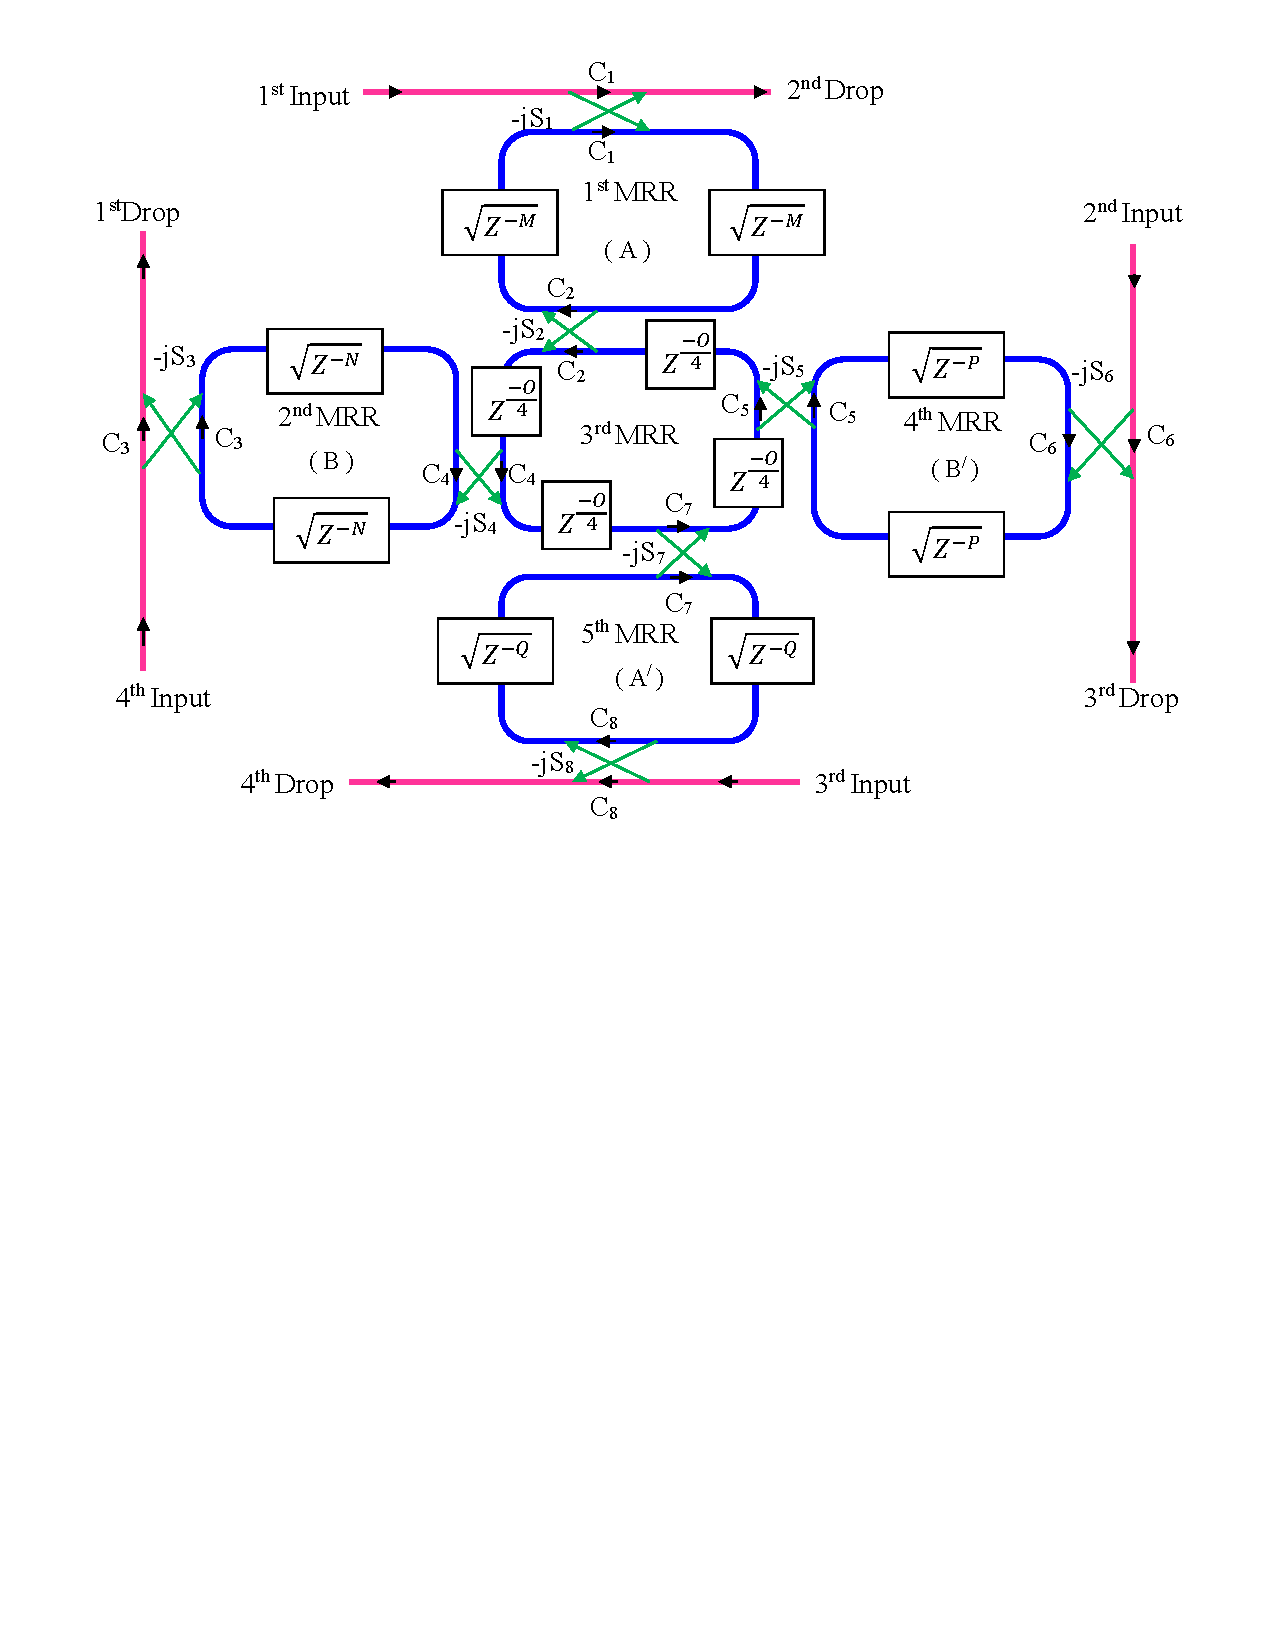
\includegraphics[width=4 in]{figs/fig1a_structure.pdf}
	\caption{Flower-like structure}
	\label{fig1a_structure}
\end{figure}
All parameters of the flower-like structure are defined as below\\
 \begin{equation}
\gamma=0 dB
\label{eqa1}
\end{equation}
 \begin{equation}
\alpha=2 dB/cm
\label{eqa2}
\end{equation}
 \begin{equation}
R_1=R_2=R_3=R_4=R_5=7.088 {\mu}m
\label{eqa3}
\end{equation}
 \begin{equation}
L_i=2{\pi}.{R_i}, i=1, 2,..., 5
\label{eqa4}
\end{equation}
 \begin{equation}
\lambda=1.55{\mu}m
\label{eqa5}
\end{equation}
 \begin{equation}
  n_{gr}=3.44
  \label{eqa6}
\end{equation}
\begin{equation}
  OPP_{MRR_{1}}=A
  \label{eqa7}
\end{equation}
  \begin{equation}
  OPP_{MRR_{2}}=B
  \label{eqa8}
\end{equation}
  \begin{equation}
  OPP_{MRR_{4}}=B'
  \label{eqa9}
\end{equation}
  \begin{equation}
  OPP_{MRR_{5}}=A'
  \label{eqa10}
\end{equation}
  \begin{equation}
  n_{effi}=n_0+(0.003).OPP_{MRR_{i}}
%n_{eff1}=3.55+(0.003).A
\label{eqa11}
\end{equation}
 %\begin{equation}
%n_{eff2}=3.55+(0.003).B
%\label{eqa7}
%\end{equation}
 %\begin{equation}
%n_{eff3}=3.55
%\label{eqa8}
%\end{equation}
 %\begin{equation}
%n_{eff4}=3.55+(0.003). B'
%\label{eqa9}
%\end{equation}
 %\begin{equation}
%n_{eff5}=3.55+(0.003). A'
%\label{eqa10}
%\end{equation}
 \begin{equation}
k_{ni}=\frac{2{\pi}.n_{effi}}{\lambda}, i=1, 2, ..., 5
\label{eqa12}
\end{equation}
 \begin{equation}
\Phi_{i}=\frac{k_{ni}.L_{i}}{2}, i=1, 2, ..., 5
\label{eqa13}
\end{equation}
 \begin{equation}
D=\sqrt{1-\gamma}
\label{eqa14}
\end{equation}
 \begin{equation}
X_{i}=D.exp(\frac{-\alpha.L_{i}}{4}), i=1, 2, ...,5
\label{eqa15}
\end{equation}
 \begin{equation}
\kappa_1=\kappa_3=\kappa_6=\kappa_8=0.1
\label{eqa16}
\end{equation}
 \begin{equation}
\kappa_2=\kappa_4=\kappa_5=\kappa_7=0.1
\label{eqa17}
\end{equation}
 \begin{equation}
S_i=D.\sqrt{\kappa_i}, i=1, 2, ..., 8
\label{eqa18}
\end{equation}
 \begin{equation}
C_i=D.\sqrt{1-\kappa_i}, i=1, 2, ..., 8
\label{eqa19}
\end{equation}
 \begin{equation}
x_i=\frac{X^2_i}{D}, i=1, 2, ..., 5
\label{eqa20}
\end{equation}
 \begin{equation}
Z_i=exp(-j.\Phi_i), i=1, 2, ..., 5
\label{eqa21}
\end{equation}
Secondly, we try to obtain transfer function for each drop port. The transfer functions have been calculated based on signal flow graph (SFG) method. In the following equations the loop gains of structure that consist of single MRR are shown:
 \begin{equation}
G_1=C_1C_2x_1Z^{-M}
\label{eqa22}
\end{equation}
 \begin{equation}
G_2=C_3C_4x_2Z^{-N}
\label{eqa23}
\end{equation}
 \begin{equation}
G_3=C_2C_4C_5C_7x_3Z^{-O}
\label{eqa24}
\end{equation}
 \begin{equation}
G_4=C_5C_6x_4Z^{-P}
\label{eqa25}
\end{equation}
 \begin{equation}
G_5=C_7C_8x_5Z^{-Q}
\label{eqa26}
\end{equation}
 \begin{equation}
G_{1,3}=-C_1C_4C_5C_7x_1x_3{S^2_2}Z^{-(M+O)}
\label{eqa27}
\end{equation}
 \begin{equation}
G_{2,3}=-C_2C_3C_5C_7x_2x_3{S^2_4}Z^{-(N+O)}
\label{eqa28}
\end{equation}
 \begin{equation}
G_{3,4}=-C_2C_4C_6C_7x_3x_4{S^2_5}Z^{-(O+P)}
\label{eqa29}
\end{equation}
 \begin{equation}
G_{3,5}=-C_2C_4C_5C_8x_3x_5{S^2_7}Z^{-(O+Q)}
\label{eqa30}
\end{equation}
 \begin{equation}
G_{1,3,5}=C_1C_4C_5C_8x_1x_3x_5{S^2_2}{S^2_7}Z^{-(M+O+Q)}
\label{eqa31}
\end{equation}
 \begin{equation}
G_{1,3,4}=C_1C_4C_6C_7x_1x_3x_4{S^2_2}{S^2_5}Z^{-(M+O+P)}
\label{eqa32}
\end{equation}
 \begin{equation}
G_{1,3,2}=C_1C_3C_5C_7x_1x_3x_2{S^2_2}{S^2_4}Z^{-(M+N+O)}
\label{eqa33}
\end{equation}
 \begin{equation}
G_{2,3,4}=C_2C_3C_6C_7x_2x_3x_4{S^2_4}{S^2_5}Z^{-(N+O+P)}
\label{eqa34}
\end{equation}
 \begin{equation}
G_{2,3,5}=C_2C_3C_5C_8x_2x_3x_5{S^2_4}{S^2_7}Z^{-(N+O+Q)}
\label{eqa35}
\end{equation}
 \begin{equation}
G_{4,3,5}=C_2C_4C_6C_8x_3x_4x_5{S^2_5}{S^2_7}Z^{-(O+P+Q)}
\label{eqa36}
\end{equation}
 \begin{equation}
G_{1,2,3,4}=-C_1C_3C_6C_7x_1x_2x_3x_4{S^2_2}{S^2_4}{S^2_5}Z^{-(M+N+O+P)}
\label{eqa37}
\end{equation}
 \begin{equation}
G_{2,3,4,5}=-C_2C_3C_6C_8x_2x_3x_4x_5{S^2_4}{S^2_5}{S^2_7}Z^{-(N+O+P+Q)}
\label{eqa38}
\end{equation}
 \begin{equation}
G_{1,3,5,2}=-C_1C_3C_5C_8x_1x_2x_3x_5{S^2_2}{S^2_4}{S^2_7}Z^{-(M+N+O+Q)}
\label{eqa39}
\end{equation}
 \begin{equation}
G_{1,3,5,4}=-C_1C_4C_6C_8x_1x_3x_4x_5{S^2_2}{S^2_5}{S^2_7}Z^{-(M+O+P+Q)}
\label{eqa40}
\end{equation}
 \begin{equation}
G_{1,2,3,4,5}=C_1C_3C_6C_8x_1x_2x_3x_4x_5{S^2_2}{S^2_4}{S^2_5}{S^2_7}Z^{-(M+N+O+P+Q)}
\label{eqa41}
\end{equation}
The determinate of graph \textit {$\Delta$} can be calculated as\\
\begin{equation}
\begin{split}
\Delta=
1-\sum_{i} {G_i}+\sum_{i,j} {G_i G_j}-\sum_{i,j,k} {G_i G_j G_k}\\+\sum_{i,j,k,l} {G_i G_j G_kG_l}-\sum_{i,j,k,l,u} {G_i G_j G_kG_lG_u} 
\label{eqa42}
\end{split}
\end{equation}
Now all RHS terms of Eq. \ref{eqa42} can be calculated as\\
\begin{equation}
\begin{split}
\sum_{i} {G_i}=G_1+G_2+G_3+G_4+G_5+G_{1,3}+G_{3,5}+G_{2,3}+\\G_{3,4}+G_{1,3,5}+G_{1,3,4}+G_{1,3,2}+G_{2,3,4}+G_{2,3,5}+G_{4,3,5}+\\G_{1,2,3,4}+G_{2,3,4,5}+G_{1,3,5,2}+G_{1,3,5,4}+G_{1,2,3,4,5} 
\label{eqa43}
\end{split}
\end{equation}

\begin{equation}
\begin{split}
\sum_{i,j} {G_i G_j}=G_1G_2+G_1G_3+G_1G_4+G_1G_5+G_1G_{2,3}+G_1G_{3,4}
+\\G_1G_{3,5}+G_1G_{2,3,4}+G_1G_{2,3,5}+G_1G_{4,3,5}+\\G_1G_{2,3,4,5}+G_2G_3+G_2G_4+G_2G_5+G_2G_{1,3}+G_2G_{3,5}+\\G_2G_{3,4}+G_2G_{1,3,5}+G_2G_{1,3,4}+G_2G_{4,3,5}+\\G_2G_{1,3,5,4}+G_3G_4+G_3G_5+G_4G_5+G_4G_{1,3}+G_4G_{3,5}+\\G_4G_{2,3}+G_4G_{1,3,5}+G_4G_{1,3,2}+G_4G_{2,3,5}+G_4G_{1,3,5,2}+\\G_5G_{1,3}+G_5G_{2,3}+G_5G_{3,4}+G_5G_{1,3,4}+G_5G_{1,3,2}+G_5G_{2,3,4}+G_5G_{1,2,3,4} 
\label{eqa44}
\end{split}
\end{equation}

\begin{equation}
\begin{split}
\sum_{i,j,k} {G_i G_j G_k}=G_1G_2G_3+G_1G_2G_4+\\G_1G_2G_5+G_1G_2G_{3,4}+G_1G_2G_{3,5}+\\G_1G_2G_{4,3,5}+G_1G_3G_4+G_1G_3G_5+G_1G_4G_5+G_1G_4G_{3,5}+\\G_1G_4G_{2,3}+G_1G_4G_{2,3,5}+G_1G_5G_{2,3}+G_1G_5G_{3,4}+\\G_1G_5G_{2,3,4}+G_2G_3G_4+G_2G_3G_5+G_2G_4G_5+G_2G_4G_{3,5}+\\G_2G_4G_{1,3}+G_2G_4G_{1,3,5}+G_2G_5G_{1,3}+G_2G_5G_{3,4}+\\G_2G_5G_{1,3,4}+G_3G_4G_5+G_4G_5G_{1,3}+G_4G_5G_{2,3}+G_4G_5G_{1,3,2} 
\label{eqa45}
\end{split}
\end{equation}

\begin{equation}
\begin{split}
\sum_{i,j,k,l} {G_i G_j G_kG_l}=G_1G_2G_3G_4+G_1G_2G_3G_5+G_1G_3G_4G_5\\
+G_1G_4G_5G_{2,3}+G_2G_3G_4G_5+G_2G_4G_5G_{1,3}+\\
G_1G_2G_4G_{3,5}+G_1G_2G_4G_5+G_1G_2G_5G_{3,4}
\label{eqa46}
\end{split}
\end{equation}

\begin{equation}
\begin{split}
\sum_{i,j,k,l,u} {G_i G_j G_kG_lG_u}=G_1G_2G_3G_4G_5 
\label{eqa47}
\end{split}
\end{equation}
The 1$^{\text{st}}$ input to the 1$^{\text{st}}$ drop port transfer function, $H_{1-1}$.\\

There is only one path from the 1$^{\text{st}}$ input to the 1$^{\text{st}}$ drop port. This is shown in Fig. \ref{fig2a_ID11}.\\
  \begin{figure}[tb]
\centering
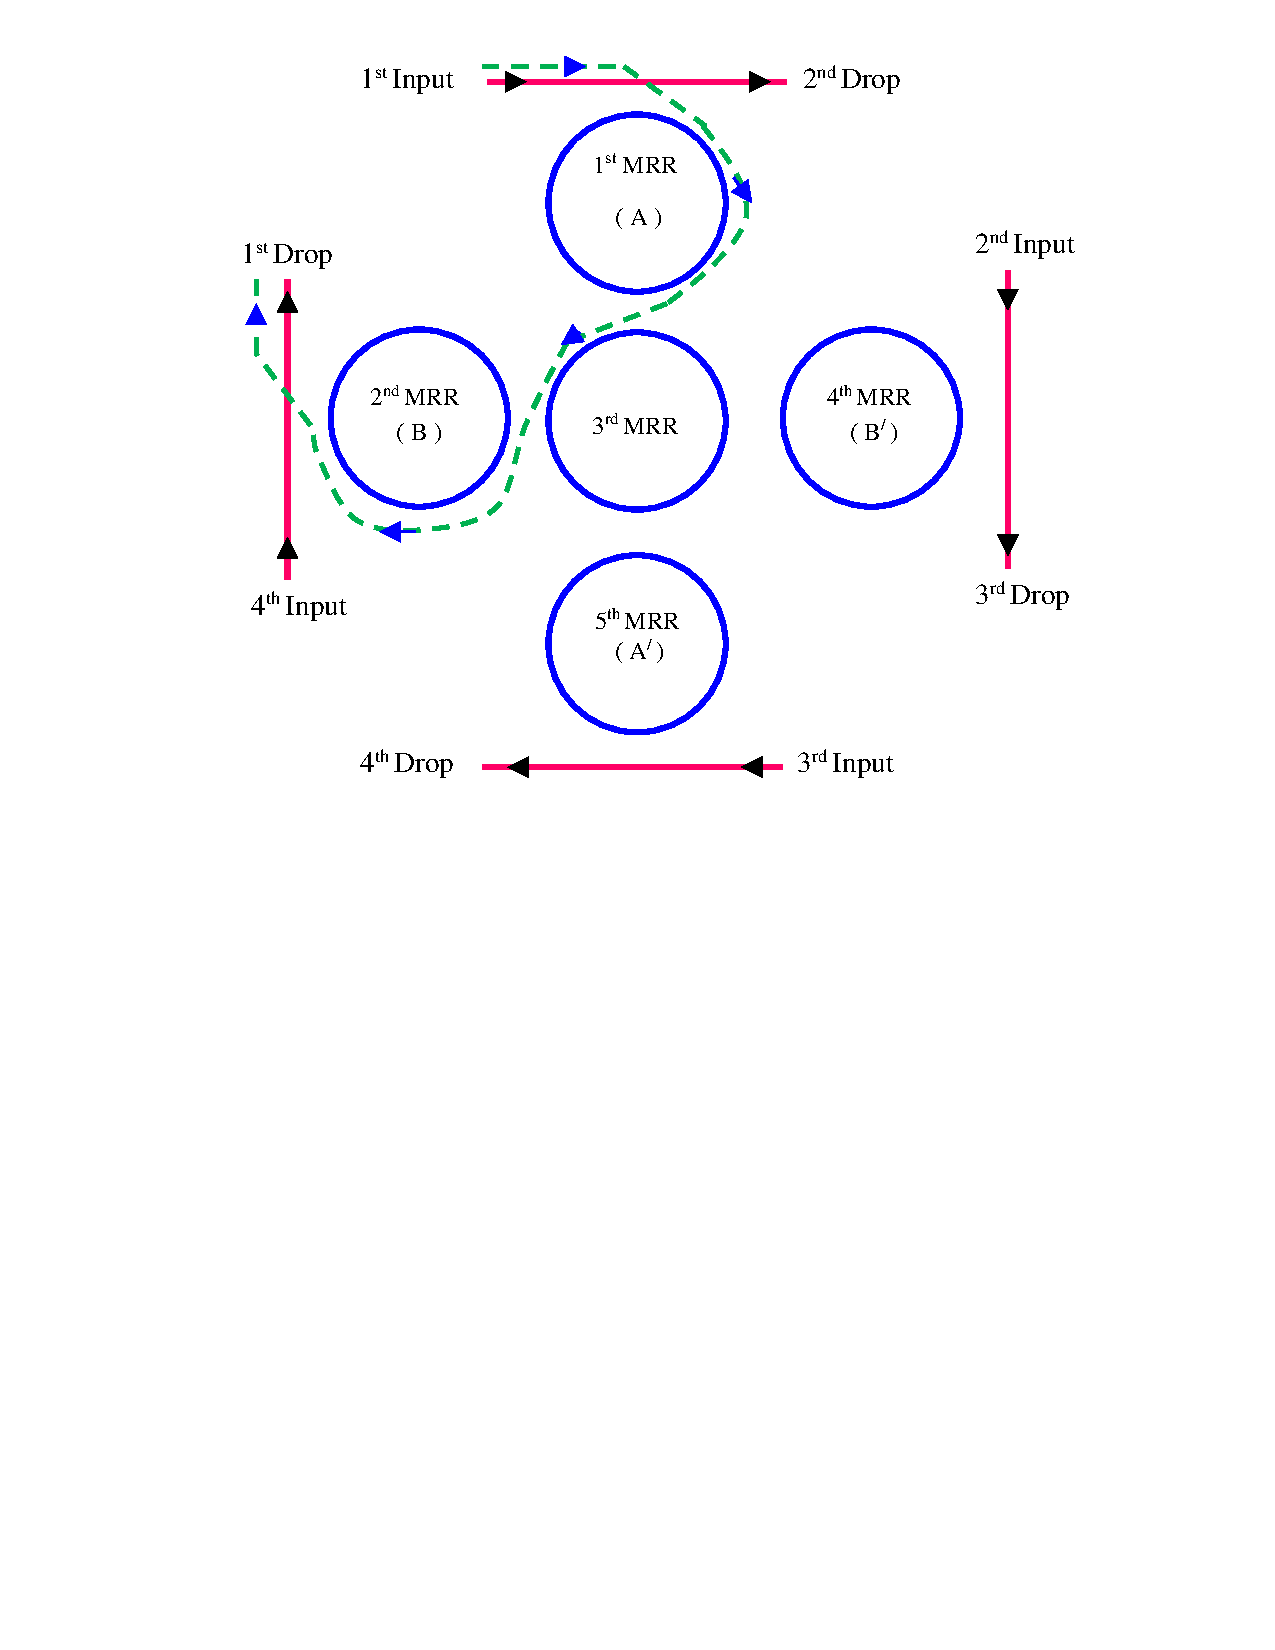
\includegraphics[width=3 in]{figs/fig2a_ID11.pdf}
	\caption{The only forward path from the 1$^{\text{st}}$ input port to the 1$^{\text{st}}$ drop port}
	\label{fig2a_ID11}
\end{figure} 
The forward path gain \textit {T} and $\Delta$ cofactor for this route is calculated as\\
\begin{equation}
\begin{split}
T_{1-1}=(-jS_{1}\sqrt{Z^{-M}})(-jS_{2}\sqrt{Z^{-\frac{-O}{2}}})(-jS_{4}\sqrt{Z^{-N}}(-jS_3)\\
=S_1S_2S_3S_4\sqrt{x_1}\sqrt{x_2}.{x^{\frac{1}{4}}_3}.Z^{\frac{-O}{4}}.Z^{\frac{-(M+N)}{2}}
\label{eqa48}
\end{split}
\end{equation}
\begin{equation}
\begin{split}
\Delta_{1-1}=1-C_5C_6Z^{-P}-C_7C_8Z^{-Q}+C_5C_6C_7C_8Z^{-(P+Q)}
\label{eqa49}
\end{split}
\end{equation}
The drop port intensity is presented as\\
\begin{equation}
\begin{split}
H_{1-1}=\frac{T_{1-1}.\Delta_{1-1}}{\Delta}
\label{eqa50}
\end{split}
\end{equation}
\begin{equation}
\begin{split}
Drop_{1-1}=H_{1-1}.E_{i1}
\label{eqa51}
\end{split}
\end{equation}

The 1$^{\text{st}}$ input to 4$^{\text{th}}$ drop port transfer function, $H_{1-4}$: 
There two paths from the 1$^{\text{st}}$ input to the 4$^{\text{th}}$ drop port. These paths are represented in Fig.\ref{fig3a}.

\begin{figure}[h!]
  \centering
    \begin{subfigure}[b]{0.4\linewidth}
    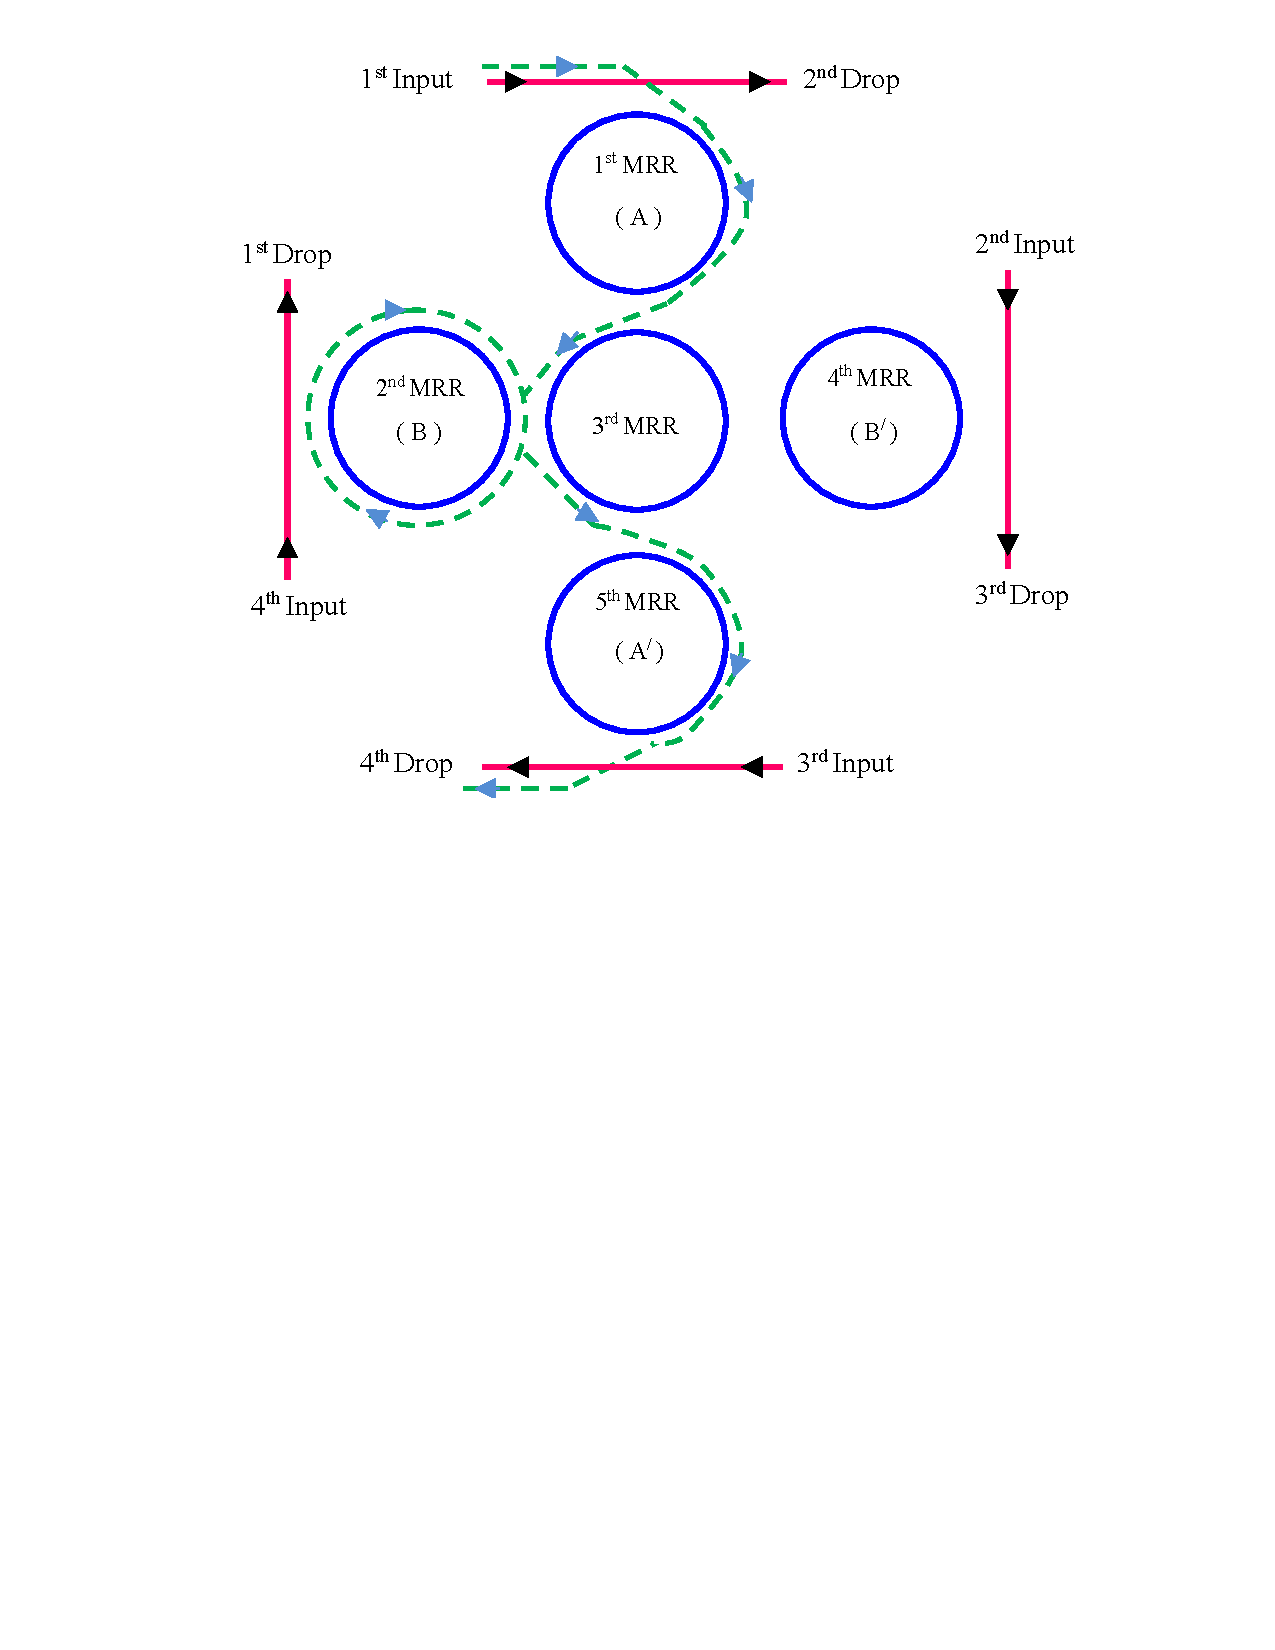
\includegraphics[width=\linewidth]{figs/fig3a_141.pdf}
    \caption{}
  \end{subfigure}
  \begin{subfigure}[b]{0.4\linewidth}
    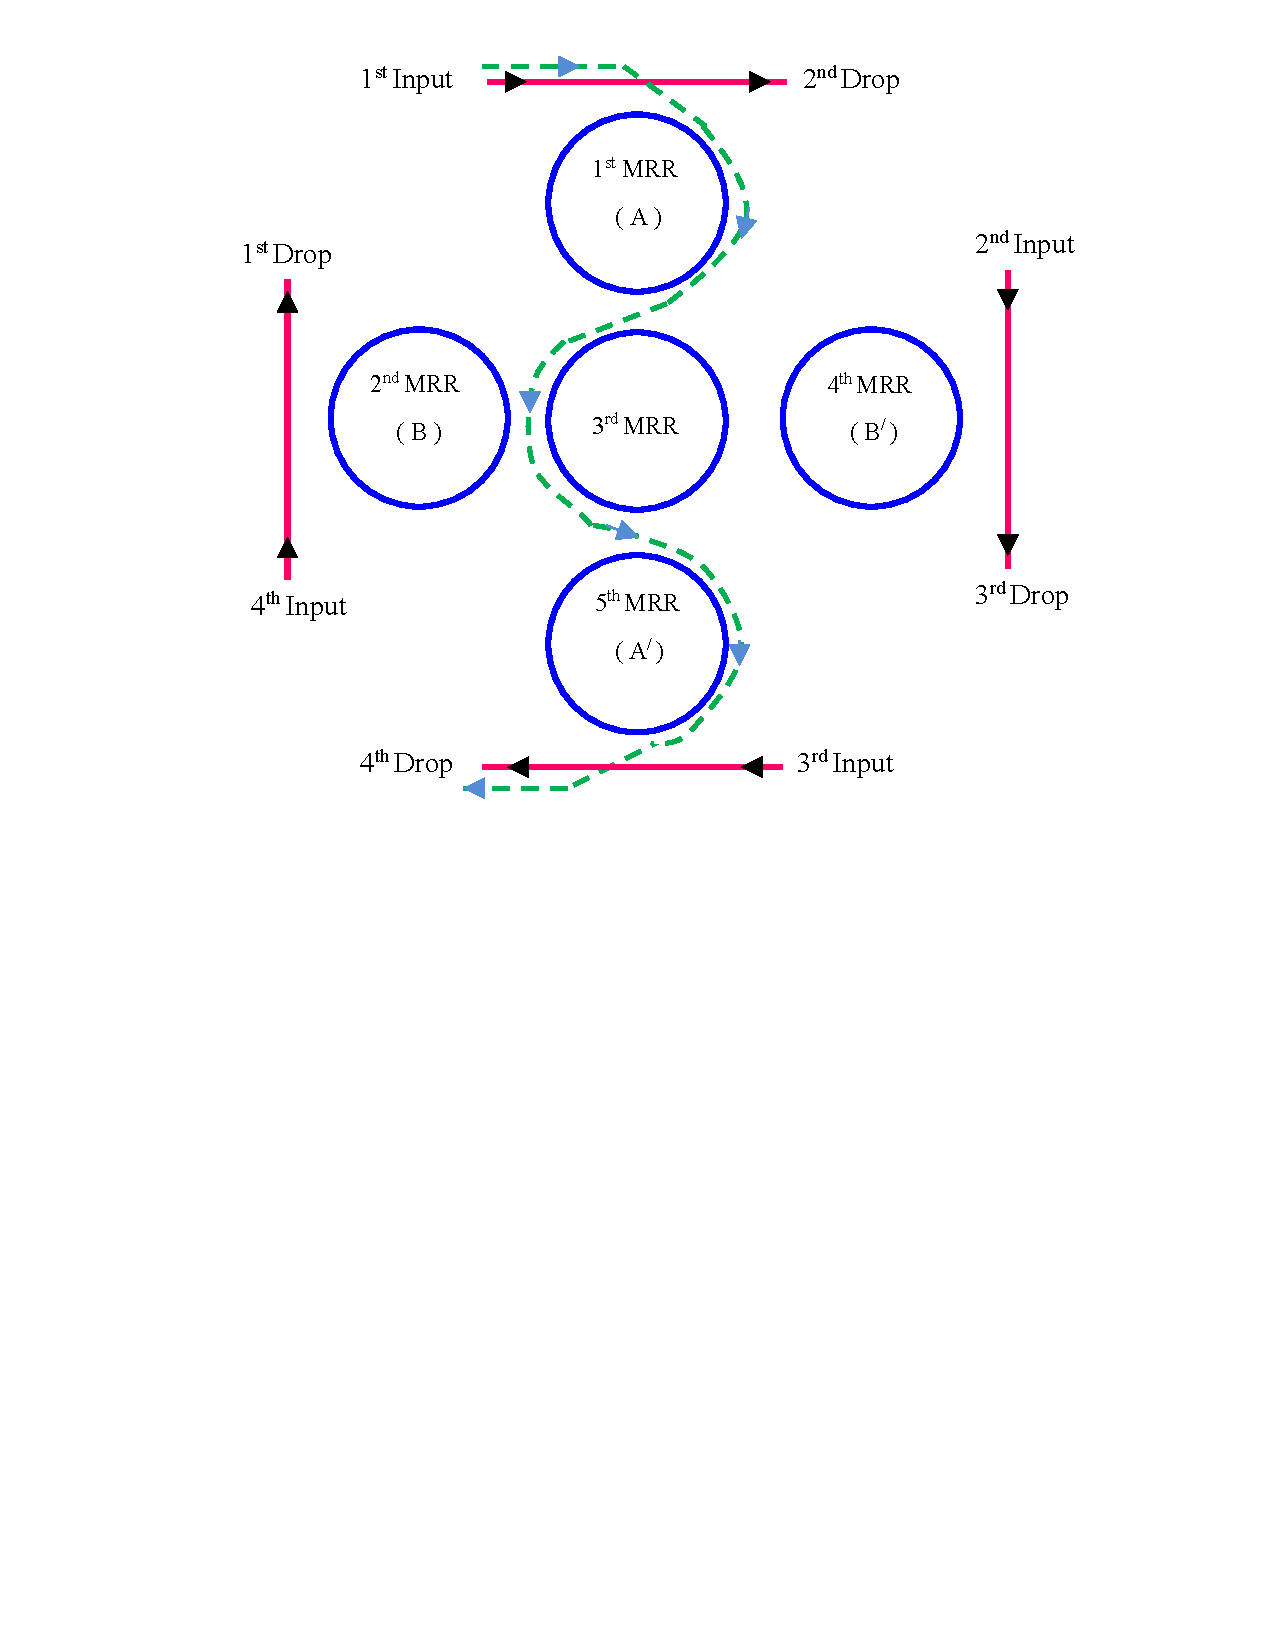
\includegraphics[width=\linewidth]{figs/fig3a_142.pdf}
    \caption{}
  \end{subfigure}
  \caption{two forward paths from the 1$^{\text{st}}$ input port to the 4$^{\text{th}}$ drop port}
  \label{fig3a}
\end{figure}

The forward path gain \textit {T} and $\Delta$ cofactor for the first route that has been depicted in Fig.\ref{fig3a}(a) can be calculated as\\

\begin{equation}
\begin{split}
T^{1^{\text{st}}}_{1-4}=-C_3S_1S_2{S^2_{4}}S_7S_8\sqrt{x_1}\sqrt{x_2}\sqrt{x_3}\sqrt{x_5}Z^{-N}\sqrt{Z^{-(M+O+Q)}}
 \label{eqa52}
\end{split}
\end{equation}

\begin{equation}
\begin{split}
\Delta^{1^{\text{st}}}_{1-4}=1-C_5C_6Z^{-P}
 \label{eqa53}
\end{split}
\end{equation}
The forward path gain \textit {T} and $\Delta$ cofactor for the second route, being presented in Fig.\ref{fig3a}(b) are calculated as

\begin{equation}
\begin{split}
T^{2^{\text{nd}}}_{1-4}=C_4S_1S_2S_7S_8\sqrt{x_1}\sqrt{x_3}\sqrt{x_5}\sqrt{Z^{-(M+O+Q)}}
\end{split}
\end{equation}

\begin{equation}
\begin{split}
\Delta^{2^{\text{nd}}}_{1-4}=1-C_3C_4Z^{-N}-C_3C_6Z^{-P}+C_3C_4C_5C_6Z^{-(N+P)}
\end{split}
\end{equation}

The drop port intensity is presented as

\begin{equation}
\begin{split}
H_{1-4}=\frac{(T^{2^{\text{nd}}}_{1-4}.\Delta^{2^{\text{nd}}}_{1-4})+(T^{1^{\text{st}}}_{1-4}.\Delta^{1^{\text{st}}}_{1-4})}{\Delta}
\end{split}
\end{equation}

\begin{equation}
\begin{split}
Drop_{1-4}=H_{1-4}.E_{i1}
\end{split}
\end{equation}

The 1$^{\text{st}}$ input to 3$^{\text{rd}}$ drop port transfer function, $H_{1-3}$\\

There are four forward paths from the 1$^{\text{st}}$ input to the 3$^{\text{rd}}$ drop port.  These four routes are illustrated in Fig.\ref{fig4a}.
\begin{figure}[h!]
  \centering
  \begin{subfigure}[b]{0.4\linewidth}
    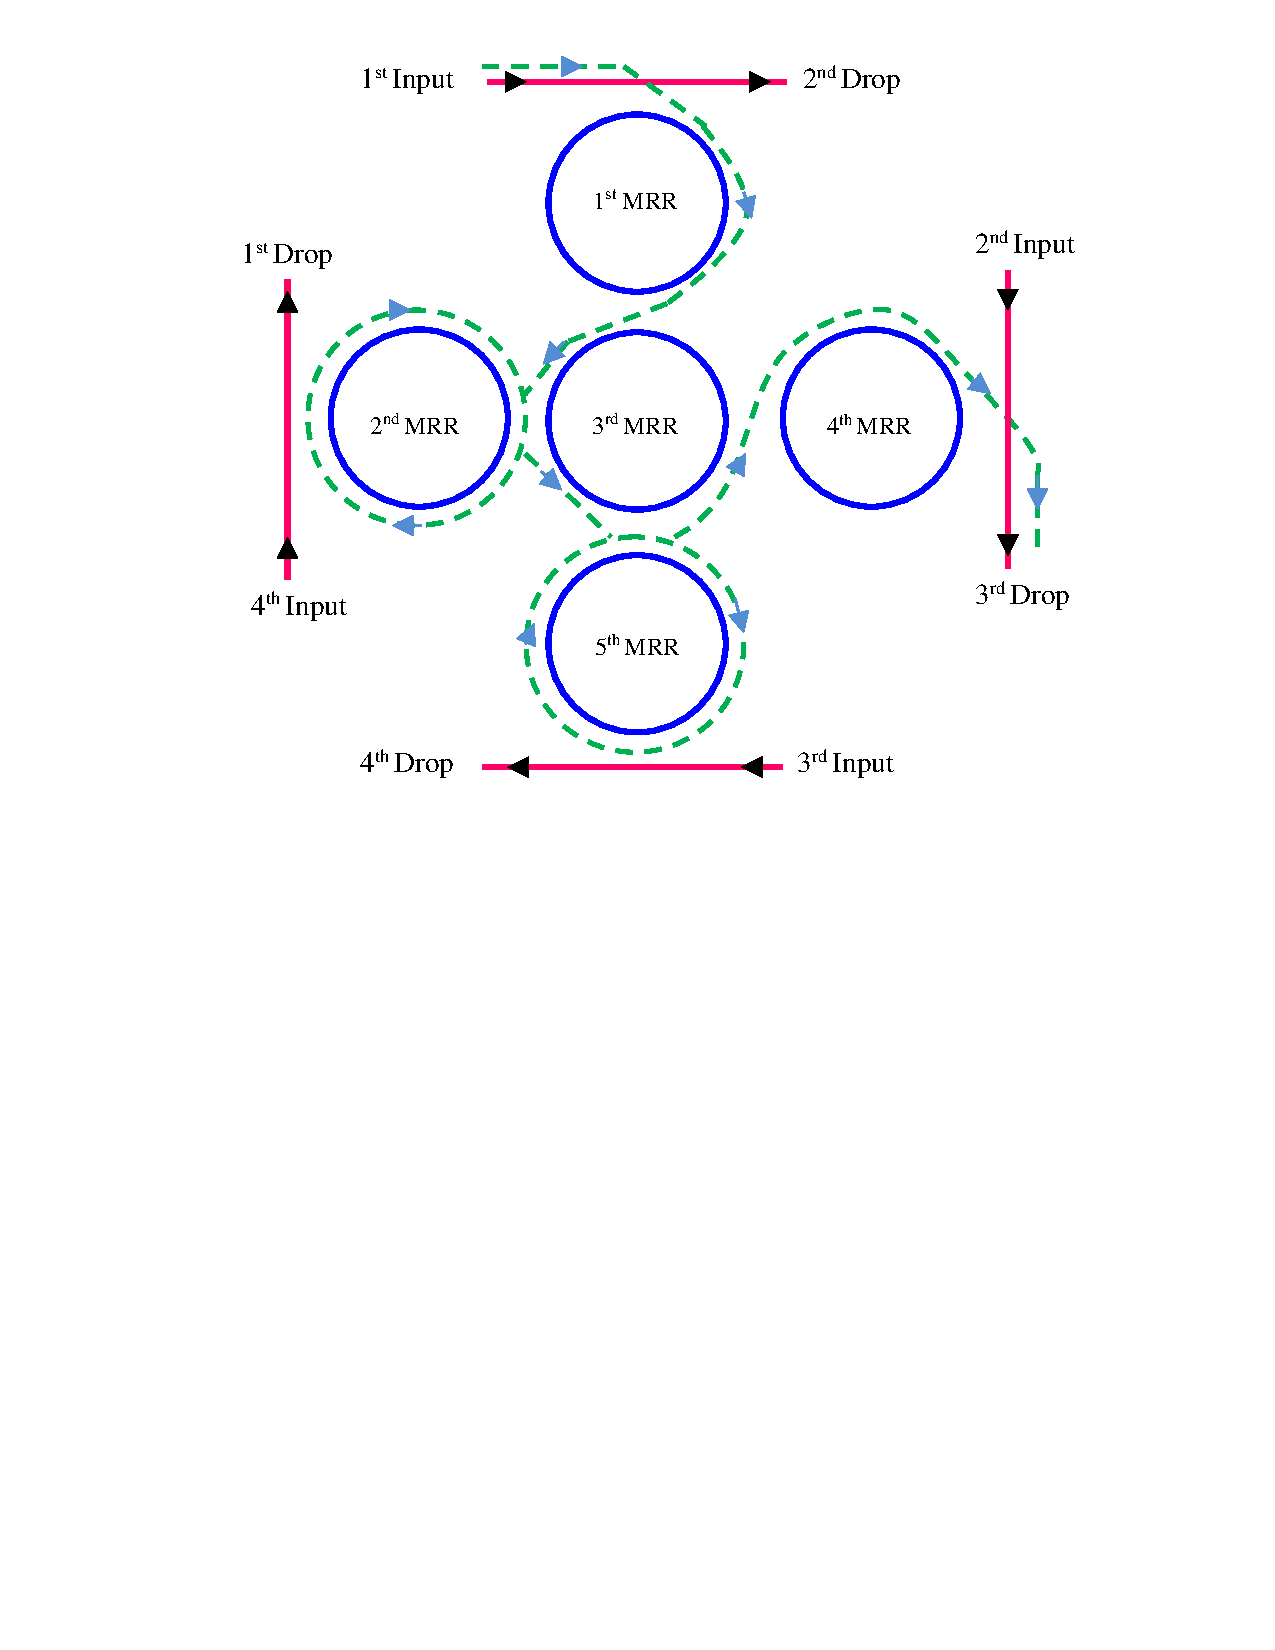
\includegraphics[width=\linewidth]{figs/fig4a_ID131.pdf}
    \caption{}
  \end{subfigure}
  \begin{subfigure}[b]{0.4\linewidth}
    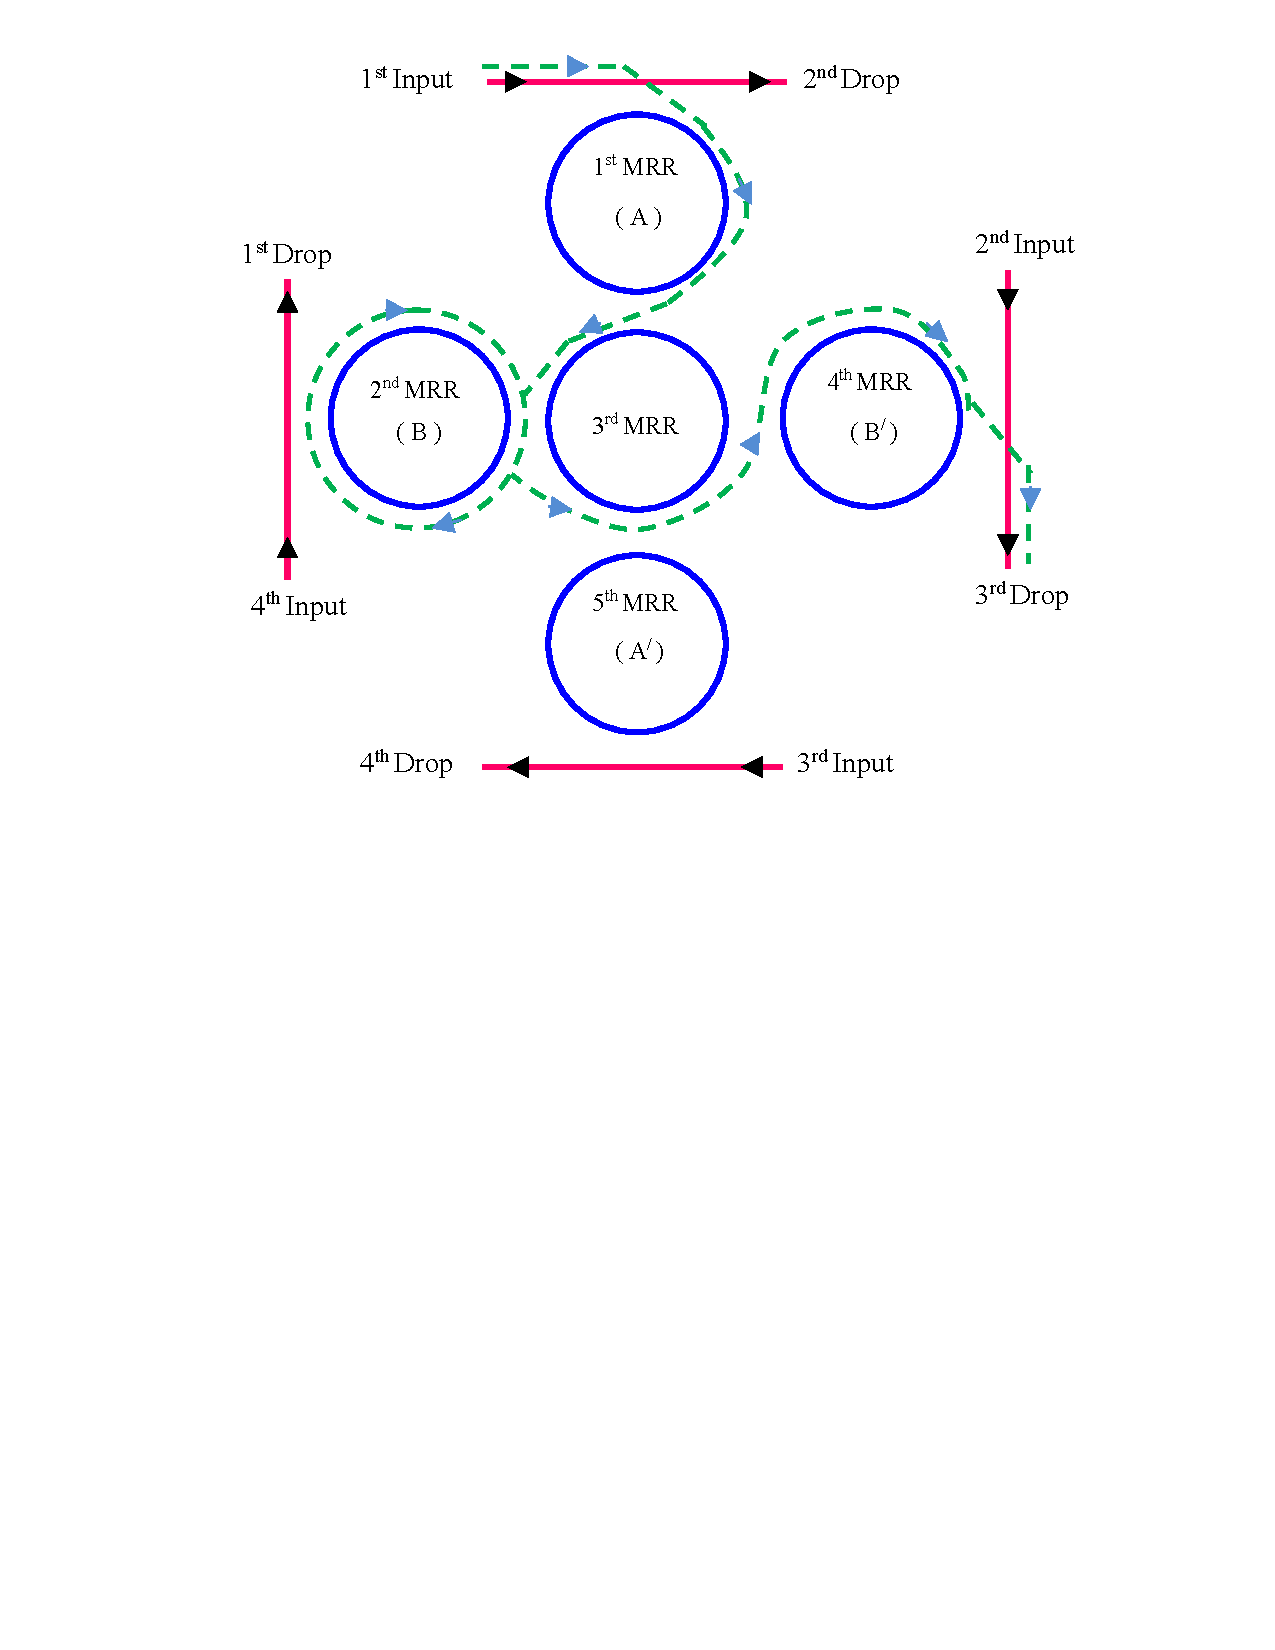
\includegraphics[width=\linewidth]{figs/fig4a_ID132.pdf}
    \caption{}
  \end{subfigure}
  \begin{subfigure}[b]{0.4\linewidth}
    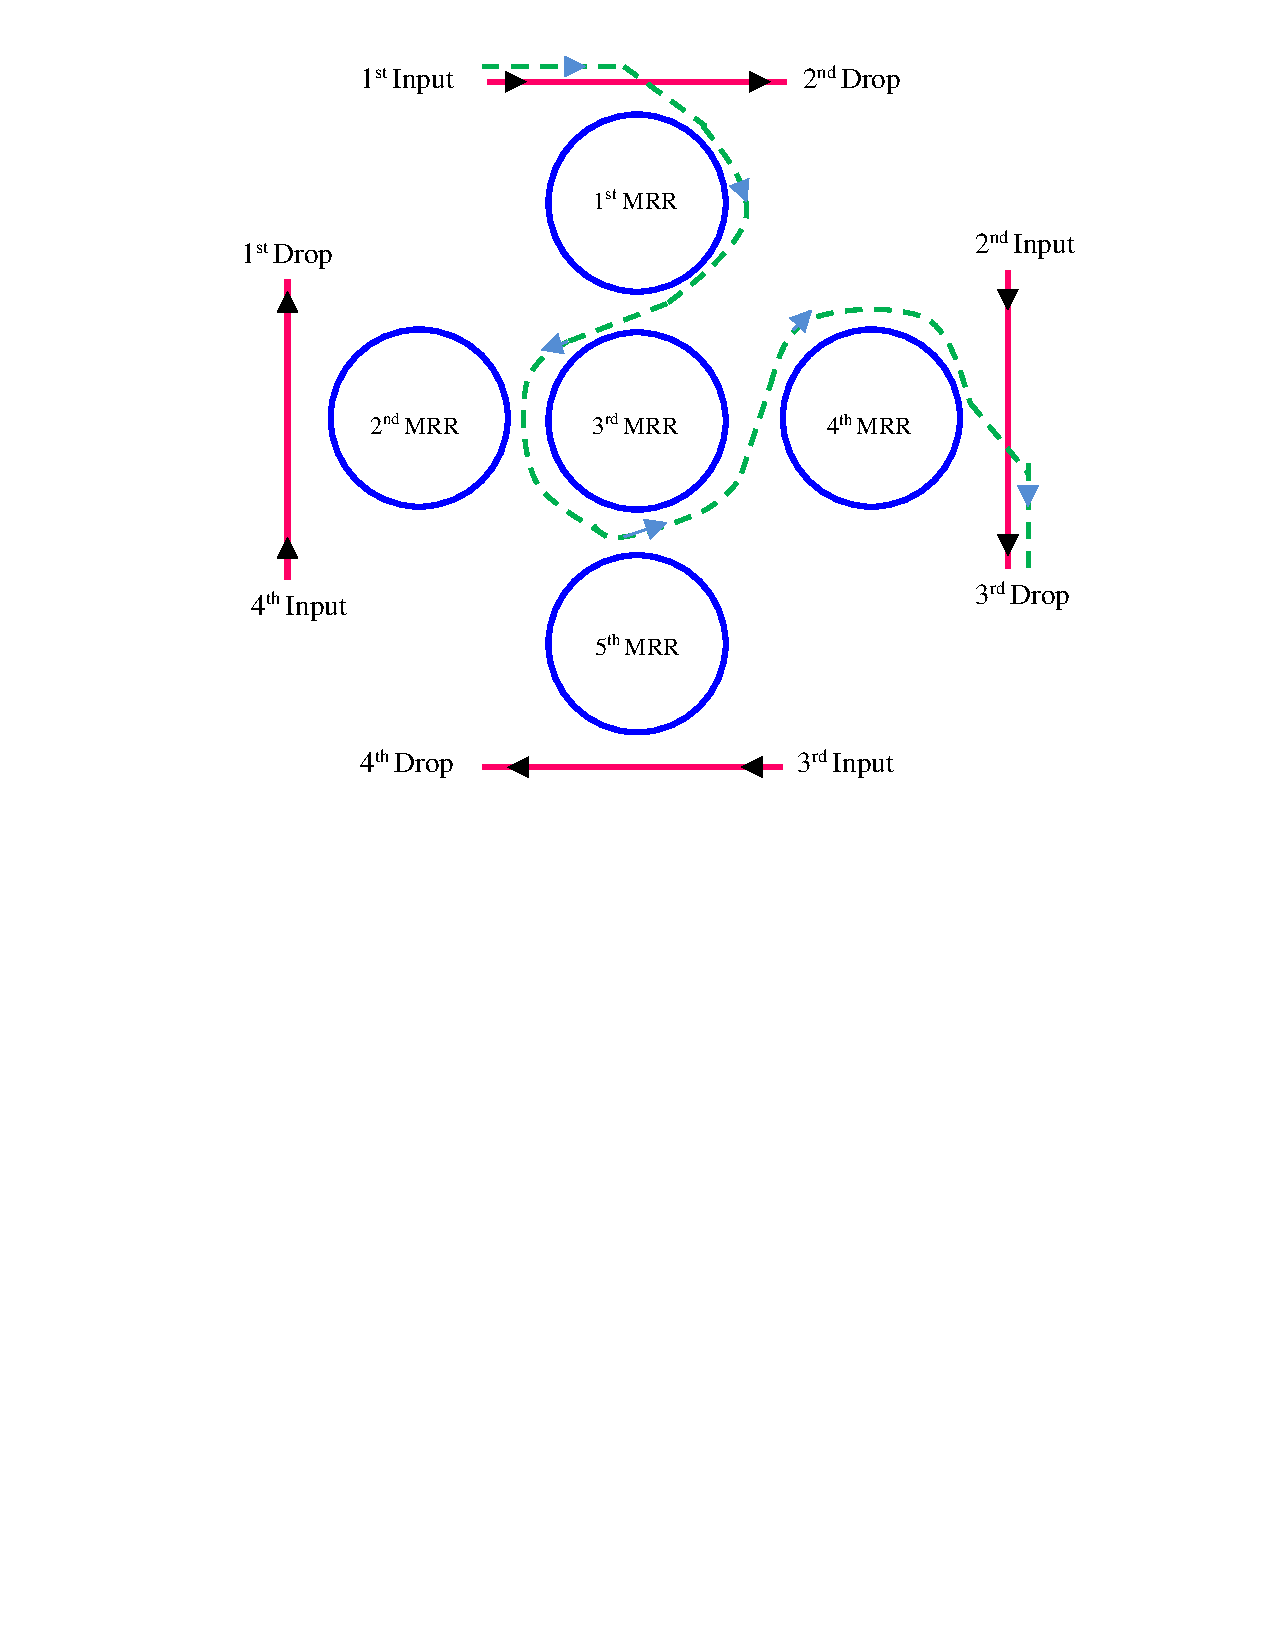
\includegraphics[width=\linewidth]{figs/fig4a_ID133.pdf}
    \caption{}
  \end{subfigure}
  \begin{subfigure}[b]{0.4\linewidth}
    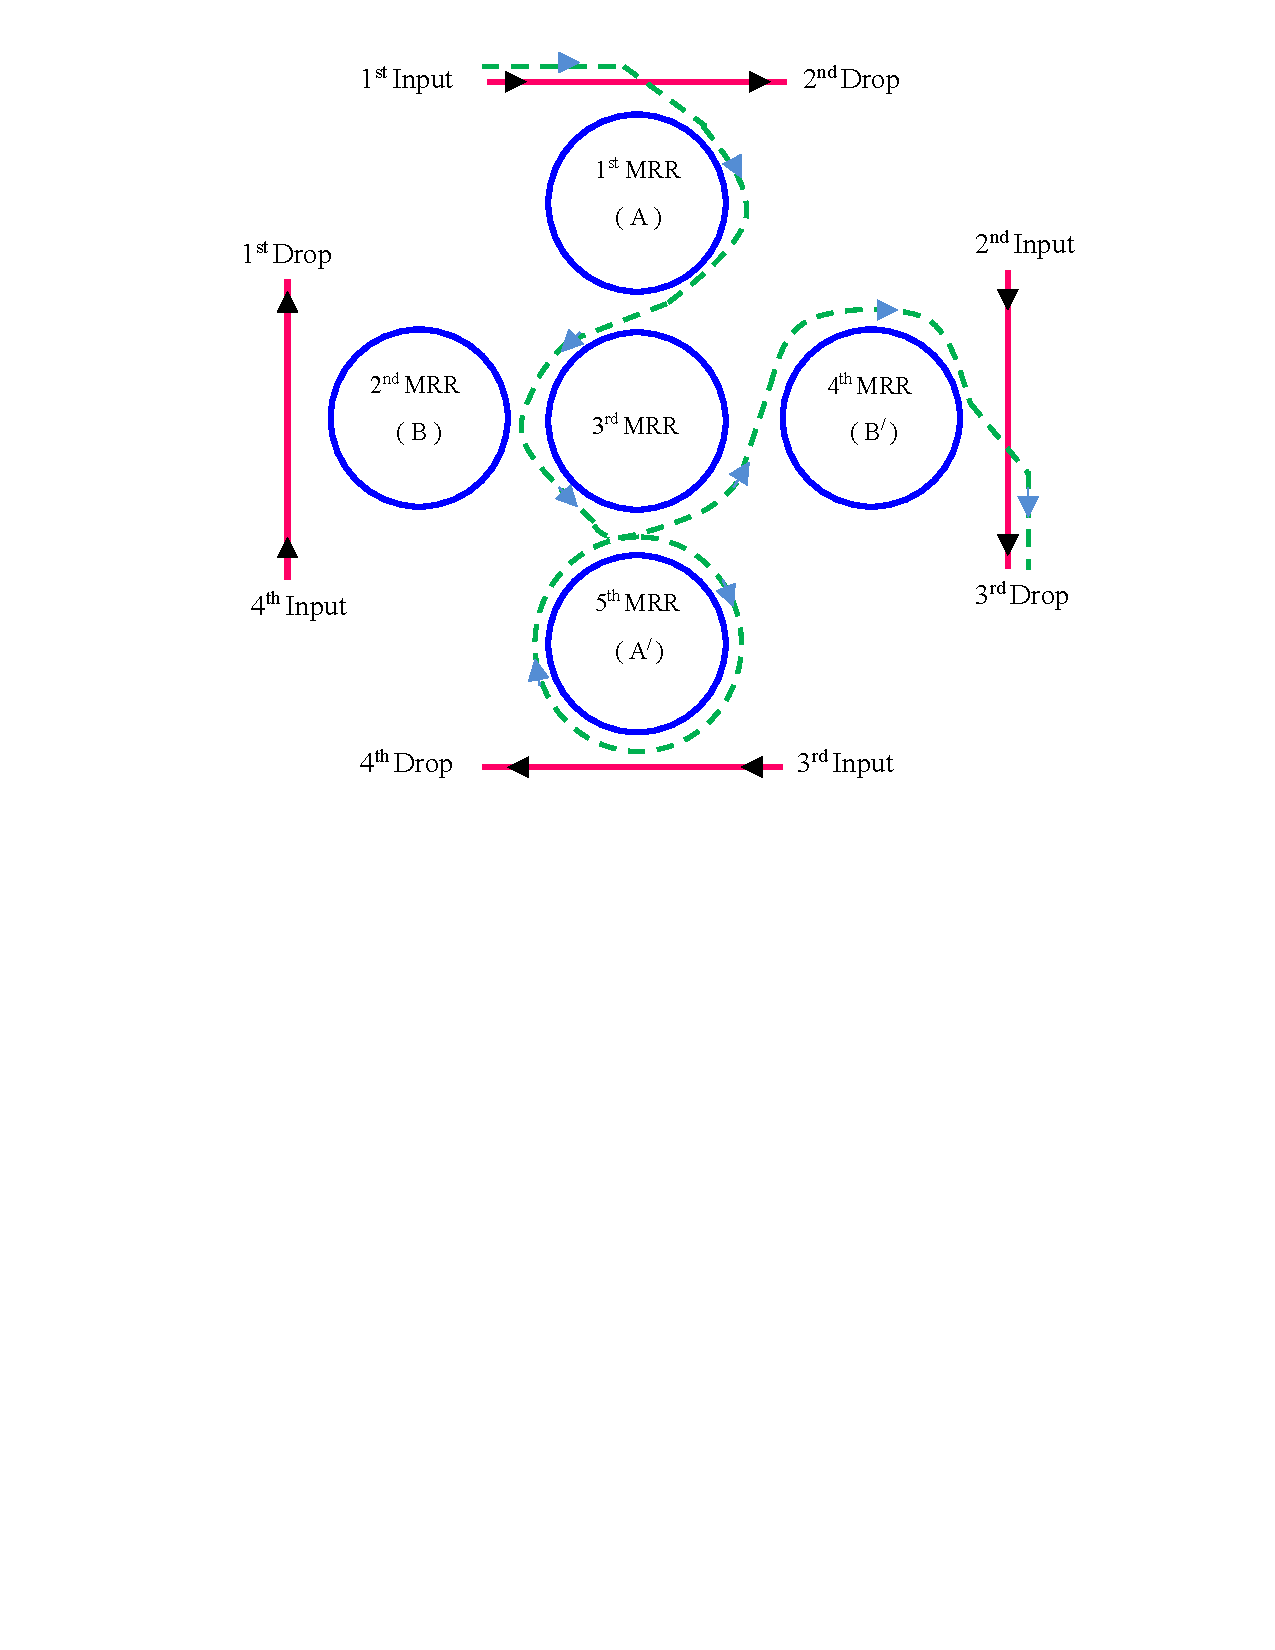
\includegraphics[width=\linewidth]{figs/fig4a_ID134.pdf}
    \caption{}
  \end{subfigure}
  \caption{all four forward paths from the 1$^{\text{st}}$ input port to the 3$^{\text{rd}}$ drop port}
  \label{fig4a}
\end{figure}
The forward path gain \textit {T} and $\Delta$ cofactor for the first route can be calculated as below. This forward path is presented in Fig.\ref{fig4a}(a).

\begin{equation}
\begin{split}
T^{1^{\text{st}}}_{1-3}=C_3C_8S_1S_2(S^2_4)S_5S_6(S^2_7)\sqrt{x_1}.x_{2}{x^{\frac{3}{4}}_3}\sqrt{x_4}.x_{5}.Z^{-(N+Q)}.\sqrt{Z^{-(M+P)}}.Z^{\frac{-3O}{4}}
\end{split}
\end{equation}

\begin{equation}
\begin{split}
\Delta^{1^{\text{st}}}_{1-3}=1
\end{split}
\end{equation}

The second forward path from the 1$^{\text{st}}$ input port to the 3$^{\text{rd}}$ drop port is represented in Fig.\ref{fig4a}(b).The forward path gain \textit {T} and $\Delta$ cofactor for this route are introduced as below

\begin{equation}
\begin{split}
T^{2^{\text{nd}}}_{1-3}=-C_3C_7S_1S_2(S^2_4)S_5S_6\sqrt{x_1}.x_{2}.{x^{\frac{3}{4}}_3}\sqrt{x_4}.Z^{-(N)}.\sqrt{Z^{-(M+P)}}.Z^{\frac{-3O}{4}}
\end{split}
\end{equation}

\begin{equation}
\begin{split}
\Delta^{2^{\text{nd}}}_{1-3}=1-C_7C_8.Z^{-Q}
\end{split}
\end{equation}
The forward path gain \textit {T} and $\Delta$ cofactor for the third route that has been depicted in Fig.\ref{fig4a}(c) are defined as

\begin{equation}
\begin{split}
T^{3^{\text{rd}}}_{1-3}=C_4C_7S_1S_2S_5S_6\sqrt{x_1}.{x^{\frac{3}{4}}_3}\sqrt{x_4}.\sqrt{Z^{-(M+P)}}.Z^{\frac{-3O}{4}}
\end{split}
\end{equation}

\begin{equation}
\begin{split}
\Delta^{3^{\text{rd}}}_{1-3}=1-C_3C_4.Z^{-N}-C_7C_8.Z^{-Q}+C_3C_4C_7C_8.Z^{-(N+Q)}
\end{split}
\end{equation}

Finally, the forth forward path from the 1$^{\text{st}}$ input port to the 3$^{\text{rd}}$ drop port is shown in Fig.\ref{fig4a}(d). The forward path gain \textit {T} and $\Delta$ cofactor are calculated as below
\begin{equation}
\begin{split}
T^{4^{\text{th}}}_{1-3}=-C_4C_8S_1S_2S_5S_6.S^2_7\sqrt{x_1}.{x^{\frac{3}{4}}_3}.\sqrt{x_4}.x_5.Z^{-Q}.\sqrt{Z^{-(M+P)}}.Z^{\frac{-3O}{4}}
\end{split}
\end{equation}

\begin{equation}
\begin{split}
\Delta^{4^{\text{th}}}_{1-3}=1-C_3C_4.Z^{-N}
\end{split}
\end{equation}

The drop port intensity is presented as
\begin{equation}
\begin{split}
H_{1-3}=\frac{(T^{1^{\text{st}}}_{1-3}.\Delta^{1^{\text{st}}}_{1-3})+(T^{2^{\text{nd}}}_{1-3}.\Delta^{2^{\text{nd}}}_{1-3})+(T^{3^{\text{rd}}}_{1-3}.\Delta^{3^{\text{rd}}}_{1-3})+(T^{4^{\text{th}}}_{1-3}.\Delta^{4^{\text{th}}}_{1-3})}{\Delta}
\end{split}
\end{equation}

\begin{equation}
\begin{split}
Drop_{1-3}=H_{1-3}.E_{i1}
\end{split}
\end{equation}

The other transfer functions can be find with the same procedure.\\


%% If you have bibdatabase file and want bibtex to generate the
%% bibitems, please use
%%
%\section*{References}
\bibliography{Refp2}
%\bibliographystyle{elsarticle-num}

%% else use the following coding to input the bibitems directly in the
%% TeX file.
%\begin{thebibliography}

%\begin{thebibliography}{70}
 
%\bibliography{refrbnn}
%\bibliographystyle{elsarticle-num}
%%% \bibitem[Author(year)]{label}
%%% Text of bibliographic item
%
%\bibitem[ ()]{}
%
%\end{thebibliography}
\end{document}
